\chapter{Homotopy Type Theory}

\section{Homotopical Language}

\begin{defn}
    A \textsl{pointed type} $(A,a)$ is a type $A\colon\univ$ together with a point $a\colon A$, called its \textsl{basepoint}. We write
    \[
        \univ_\sbull\defeq\sum_{A:\,\univ}A
    \]
    for the type of pointed types in the universe $\univ$.
\end{defn}

\begin{defn}
    Given a pointed type $(A,a)$, we define the \textsl{loop space} of $(A,a)$ to be the following pointed type:
    \[
        \Omega(A,a)\defeq((a\eq Aa),\fun{refl}_a).
    \]
    An element of this type is called a \textsl{loop} at $a$. For $n\colon\N$, the \textsl{$n$-fold iterated loop space} $\Omega^n(A,a)$ of a pointed type $(A,a)$ is defined recursively by:
    \begin{align*}
        \Omega^0(A,a)&\defeq(A,a)\\
        \Omega^{n+1}(A,a)&\defeq\Omega^n(\Omega(A,a)).
    \end{align*}
    An element of this type is called an \textsl{$n$-loop} or an \textsl{$n$-dimensional loop} at $a$.

    Note that $\Omega^1(A,a)\equiv\Omega(A,a)$.
\end{defn}

\begin{rem}
    Recall from Exercise~\ref{exr:ap-application} that given $f\colon A\to B$, the congruence function
    \[
        \fun{ap}_f\colon\prod_{x,y\colon A}\;\prod_{p\colon x\eq Ay}f(x)\eq Bf(y)
    \]
    transforms paths in $A$ to paths in $B$. Specifically
    \[
        \fun{ap}_f(x,y,p)\colon f(x)\eq Bf(y),\quad\text{for }p\colon x\eq Ay,
    \]
    where the notation $\fun{ap}_f(x,y,p)$ is usually simplified to $\fun{ap}_f(p)$ or $\tilde f(p)$.
\if{false}    
    Moreover,
    \[
        \fun{ap}_f(\fun{refl}_x)\equiv\fun{refl}_{f(x)}
        \quad\text{and}\quad
        \fun{ap}_f(p\ct q)\eq{f(x)\eq Bf(z)}
            \fun{ap}_f(p)\ct \fun{ap}_f(q).
    \]
\fi
\end{rem}

\begin{prop}\label{prop:ap-properties}
    Let $A,B,C\colon\univ$. Given functions\/ $f\colon A\to B$ and\/ $g\colon B\to C$ and paths\/ $p\colon x\eq Ay$ and\/ $q\colon y\eq Az$, we have:
    \begin{enumerate}[a),font=\upshape]
        \item $\tilde f(\fun{refl}_x)\equiv\fun{refl}_{f(x)}$.
        \item $\tilde f(p\ct q)\eq{f(x)\eq Bf(z)}\tilde f(p)\ct\tilde f(q)$.
        \item $\tilde f(p^{-1})\eq{f(y)\eq Bf(x)}\tilde f(p)^{-1}$.
        \item $\tilde g(\tilde f(p))\eq{h(x)\eq Ch(y)}\tilde h(p)$, where $h\defeq g\circ f$.
        \item $\widetilde{\id}_A(p)\eq{x\eq Ay}p$.
    \end{enumerate}
\end{prop}

\begin{proof}${}$
    \begin{enumerate}[a)]
        \item Exercise~\ref{exr:ap-application}.
        \item Exercise~\ref{exr:ap-application}.
        
        \item First observe that
        \begin{align*}
            \tilde f(p)\ct\tilde f(p^{-1})
                &\eq{f(x)\eq Bf(x)}\tilde f(p\ct p^{-1})
                    &&\text{; by part b)}\\
                &\eq{f(x)\eq Bf(x)}\tilde f(\fun{refl}_x)
                    &&\text{; inverse law}\\
                &\equiv\fun{refl}_{f(x)}
                    &&\text{; by part a).}
        \end{align*}
        Therefore,
        \begin{align*}
            \tilde f(p)^{-1}
                &\eq{f(y)\eq Bf(x)}
                    \tilde f(p)^{-1}\ct\big(\tilde f(p) \ct\tilde f(p^{-1})\big)
                    &&\text{; right unit}\\
                &\eq{f(y)\eq Bf(x)}
                    \big(\tilde f(p)^{-1}\ct\tilde f(p)\big) \ct\tilde f(p^{-1})
                    &&\text{; associativity}\\
                &\eq{f(y)\eq Bf(x)}\tilde f(p^{-1})
                    &&\text{; left inverse.}
        \end{align*}

        \item Since $p\colon x\eq Ay$, we know that $\tilde f(p)\colon f(x)\eq Bf(y)$. Therefore,
        \[
            \tilde g(\tilde f(p))\colon g(f(x))\eq Cg(f(y)).
        \]
        Let $h\defeq g\circ f$. Note that the type of the term above is definitionally equal to $h(x)\eq C h(y)$.
        Consider the case where $p\equiv\fun{refl}_x$. We have
        \begin{align*}
            \tilde g(\tilde f(\fun{refl}_x))
                &\equiv \tilde g(\fun{refl}_{f(x)})\\
                &\equiv \fun{refl}_{g(f(x))}\\
                &\equiv \fun{refl}_{h(x)}\\
                &\equiv \tilde h(\fun{refl}_x).
        \end{align*}
        To conclude that $\tilde g(\tilde f(p))\eq{h(x)\eq Ch(y)}\tilde h(p)$, we apply path induction to the motive
        \[
            C(x,y,p)\defeq \tilde g(\tilde f(p))\eq{h(x)\eq Ch(y)}\tilde h(p),
        \]
        with the base case $c(x)\colon C(x,x,\fun{refl}_x)$ defined as $\fun{refl}_{\tilde h(\fun{refl}_x)}$.

        \item For\/ $p\equiv\fun{refl}_x$, since\/ $\id_A(x)\equiv x$, we have
        \begin{align*}
            \widetilde{\id}_A(\fun{refl}_x)
                &\equiv \fun{refl}_{\id_A(x)}\\
                &\equiv \fun{refl}_x.
        \end{align*}
        Therefore, the conclusion follows by path induction applied to the motive
        \[
            C(x,y,p)\defeq\widetilde{\id}_A(p)\eq{x\eq Ay}p
        \]
        with base case\/ $c(x)\defeq\fun{refl}_{\fun{refl}_x}\colon C(x,x,\fun{refl}_x)$.
        
    \end{enumerate}
\end{proof}

\begin{lem}\label{lem:ap-const}
    Let\/ $A, B\colon\univ$ and\/ $b\colon B$. Given the constant function\/ $f\colon A\to B$ defined by\/ $f(x)\defeq b$, for any path\/ $p\colon x\eq A y$, we have
    \[
        \fun{ap}_f(p) \eq{b\eq B b} \fun{refl}_b.
    \]
\end{lem}

\begin{proof}
    By path induction on $p$ it suffices to prove the case where $y\equiv x$ and $p\equiv \fun{refl}_x$.
    \begin{enumerate}[-]
        \item \lhs: $\fun{ap}_f(\fun{refl}_x)\equiv\fun{refl}_{f(x)}\equiv \fun{refl}_b$.
        \item \rhs: $\fun{refl}_b$.
    \end{enumerate}
    Since both sides are definitionally equal to $\fun{refl}_b$, the equality is inhabited by $\fun{refl}_{\fun{refl}_b}$.
\end{proof}

\begin{rem}\label{rem:fibration}
    Recall from classical topology that a \textsl{fibration} is a continuous map $\pi\colon E\to B$ with the homotopy-lifting property:
    \[
        \begin{tikzcd}[row sep=large, column sep=huge]
            X
                \arrow[r,"f"]
                \arrow[d,hook,"i_0"']
            &E
                \arrow[d,"\pi"] \\
            X\times I
                \arrow[r,"\forall H"']
                \arrow[ur,dashed,"\exists\tilde{H}"]
            &B
        \end{tikzcd}
    \]
    In this context, $E$ is the \textsl{total space}\footnote{After the French \textit{Espace}.} and $B$ the \textsl{base space} of the fibration.

    \textsl{Serre fibrations} lift paths, path homotopies, and higher-dimensional volumes. For instance, in the case of paths, the diagram above becomes:
    \[
        \begin{tikzcd}[row sep=large, column sep=large]
            \{0\}
                \arrow[r, "e_0"]
                \arrow[d, hook, "i"']
            & E
                \arrow[d, "\pi"] \\
            I
                \arrow[r, "\forall\gamma"']
                \arrow[ur, dashed, "\exists\tilde{\gamma}"]
            & B
        \end{tikzcd}
    \]
    In Homotopy Type Theory, given a type family $P\colon A\to\univ$, the first projection $\fun{\pi}_1\colon \sum_{x\colon A}P(x)\to A$ is analogous to a fibration with \textsl{total space} $\sum_{x\colon A}P(x)$ and \textsl{base space} $A$. This structural analogy is established by the lemma below.

    Given $a,b\colon A$, the type family $P$ structurally relates the fibers $P(a)$ and $P(b)$. Although a point $u\colon P(a)$ cannot be directly compared with $v\colon P(b)$ due to type mismatch, it is possible to establish a connection between the pairs $(a,u)$ and $(b,v)$ within the $\Sigma$-type. Specifically, if there exists a path $p\colon a\eq A b$, we can transport $u$ along $p$ to obtain an element $\fun{transport}^P(p,u)\colon P(b)$. Since this transported term inhabits the same fiber as $v$, the comparison becomes well-defined. More precisely:
    
\end{rem}

\begin{thm}{\upshape[Path Lifting Property]}\label{thm:path-lift}
    Let\/ $P\colon A\to\univ$ be a type family over\/~$A$ and let\/ $E\defeq\sum_{x\colon A}P(x)$ be its total space. Given $a,b\colon A$, there exists a function
    \[
        \fun{lift}\colon\prod_{u\colon P(a)}\;
            \prod_{p\colon a\eq Ab}
            (a,u)\eq{E}(b,\fun{transport}^P(p,u))
    \]
    \needspace{2\baselineskip}
    satisfying the following properties:
    \begin{enumerate}[i), font=\upshape]
        \item $\fun{lift}(u,p)\colon (a,u)\eq E (b,\fun{transport}^P(p,u))$.
        \item $\fun{lift}(u,\fun{refl}_a)\equiv\fun{refl}_{(a,u)}$.
        \item $\fun{ap}_{\pi_1}(\fun{lift}(u,p))\eq{a\eq Ab}p$.
    \end{enumerate}
    where\/ $\pi_1\colon E\to A$ denotes the first projection.\footnotemark
\end{thm}
\footnotetext{Since\/ $\pi_1$ maps the total space to the base type\/ $A$, the functorial action\/ $\fun{ap}_{\pi_1}$ projects paths in\/ $E$ to paths in\/ $A$.}


\begin{proof}
    Consider the motive family\/ $C\colon\prod_{x\colon A}(a\eq Ax)\to\univ$, defined by
    \[
        C(x,p)\defeq(a,u)\eq E(x,\fun{transport}^P(p,u)).
    \]
    Since\/ $\fun{transport}^P(\fun{refl}_a,u)\equiv u$, we have
    \[
        C(a,\fun{refl}_a)\equiv(a,u)\eq E(a,u),
    \]
    and we can specify the base case\/ $c\defeq\fun{refl}_{(a,u)}$ to define, by \nref{lpar:based-path-induction},
    \[
        \fun{lift}(u,p)\defeq\fun{ind}'_{\eq A}(a,C,c,x,p).
    \]
    We can use based path induction again to verify that
    \[
        \fun{ap}_{\fun{\pi}_1}(\fun{lift}(u,p)) \eq{a\eq Ax} p.
    \]
    For the base case, we know definitionally that\/ $\fun{lift}(u,\fun{refl}_a) \equiv \fun{refl}_{(a,u)}$. Thus,
    \[
        \fun{ap}_{\fun{\pi}_1}(\fun{lift}(u,\fun{refl}_a))
        \equiv \fun{ap}_{\fun{\pi}_1}(\fun{refl}_{(a,u)})
        \equiv \fun{refl}_{\pi_1(a,u)}
        \equiv \fun{refl}_a.
    \]
\end{proof}

\begin{rem}\label{rem:section-type}
    The lemma can be represented by the following diagram, where the horizontal arrows represent paths ---i.e., terms of the propositional equalities between their ends--- and the vertical arrows, functions:
    \[
        \begin{tikzcd}[row sep=large, column sep=huge]
            (a,u)
                \arrow[r,"{\fun{lift}(u,p)}"]
                \arrow[d,"\pi_1"']
            &(x, \fun{transport}^P(p,u))
                \arrow[d,"\pi_1"] \\
            a
                \arrow[r,"p"']
            &x
        \end{tikzcd}
        \qquad;\ u\colon P(a),\;p\colon a\eq Ax.
    \]
    Note also that a term $f\colon\prod_{x\colon A}P(x)$ can be regarded as a \textsl{section} of the fibration induced by~$P$.
\end{rem}

\begin{ntn}\label{ntn:p_*}
    When\/ $P$ is clear from the context we will simply write
    \[
        p_*(u)\defeq\fun{transport}^P(p,u)\colon P(x).
    \]
    In particular,
    \begin{equation}\label{eq:refl-*}
        (\fun{refl}_a)_*(u)\equiv u.
    \end{equation}
\end{ntn}

\begin{defn}\label{defn:sec}
    Let $A,B\colon\univ$. Given $b\colon B$ we define the \textsl{section} function
    \[
        \fun{sec}_b\colon A\to A\times B,\quad a\mapsto(a,b).
    \]
    Note that
    \begin{align*}
        \pi_1\circ\fun{sec}_b
            &\equiv\pi_1(\lambda x.\,(x,b))
            \equiv\lambda x.\,\pi_1((x,b))
            \equiv\lambda x.\,x
            \equiv\id_A.\\
        \pi_2\circ\fun{sec}_b
            &\equiv\pi_2(\lambda x.\,(x,b)
            \equiv\lambda x.\,\pi_2((x,b)
            \equiv\lambda x.\,b.
    \end{align*}
\end{defn}

\begin{rem}\label{rem:sec-lift}
    In the particular case where $P$ is a constant family $P(x)\equiv B$ for $x\colon A$, given $p\colon a\eq Aa'$, we have
    \begin{enumerate}[i)]
        \item $\fun{lift}(b,p)\eq{(a,b)\eq{A\times B}(a',b)}\fun{ap}_{\fun{sec}_b}(p)$,
        \item $\fun{lift}(b,\fun{refl}_a)\equiv\fun{refl}_{(a,b)}$, and
        \item $\fun{ap}_{\pi_1}(\fun{lift}(b,p))\eq{a\eq Aa'}p$.
    \end{enumerate}
    In fact, the equality of part~i) follows from part~ii) by induction on $p$.
    \[
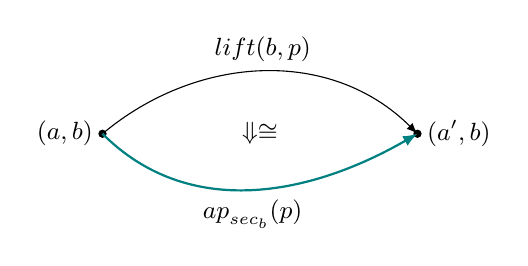
\begin{tikzpicture}[scale=1, >=stealth, font=\small]
    % Points
    \coordinate (start) at (0,0);
    \coordinate (end) at (4,0);

    \fill (start) circle (1.5pt) node[left] {$(a,b)$};
    \fill (end) circle (1.5pt) node[right] {$(a',b)$};

    % Top Path: lift(b,p)
    \draw[-latex,] (start) to[out=40, in=135] 
        node[midway, above,black] {$\fun{lift}(b,p)$} (end);

    % Bottom Path: ap(sec_b, p)
    \draw[-latex, thick, teal] (start) to[out=-45, in=-150] 
        node[midway, below,black] {$\fun{ap}_{\fun{sec}_b}(p)$} (end);

    % The 2-path (Equality)
    \node at (2,0) {$\Downarrow \cong$};
\end{tikzpicture}
    \]
\end{rem}

\begin{lem}{\upshape[Dependent map]}\label{lem:dependent-map}
    Let\/ $P\colon A\to\univ$. If\/ $f\colon\prod_{x\colon A}P(x)$, then there is a map
    \[
        \fun{apd}_f\colon\prod_{x,y\colon A}\;
            \prod_{p\colon x\eq Ay}
                p_*(f(x))\eq{P(y)}f(y)
    \]
    satisfying $\fun{apd}_f(\fun{refl}_x)\equiv\fun{refl}_{f(x)}$.
\end{lem}

\begin{proof}
    Fix $a\colon A$ and consider the motive
    \begin{align*}
        C&\colon\prod_{a\colon A}(a\eq Ax)\to\univ\\
        C(x,p)&\defeq p_*(f(a))\eq{P(x)}f(x).
    \end{align*}
    Since
    \begin{align*}
        C(a,\fun{refl}_a)
            &\equiv (\fun{refl}_a)_*(f(a))\eq{P(a)}f(a)\\
            &\equiv f(a)\eq{P(a)}f(a)
                &&\text{; \eqref{eq:refl-*}},
    \end{align*}
    we can specify $c\defeq\fun{refl}_{f(a)}$ and obtain $\fun{apd}_f$ by based path induction.
\end{proof}

\begin{lem}\label{lem:constant-fibration}
    If\/ $P \colon A \to \univ$ is defined by\/ $P(x) :\equiv B$ for a fixed\/ $B \colon \univ$, then for any\/ $x, y \colon A$ and\/ $p \colon x \eq A y$ and\/ $b \colon B$ we have a path
    \[
        \fun{transportconst}^B_p(b) \colon \fun{transport}^P(p, b) \eq B b
    \]
    satisfying\/ $\fun{transportconst}^B_{\fun{refl}_x}\defeq\lambda b.\,\fun{refl}_b$.
\end{lem}

\begin{proof}
    See Exercise \ref{exr:constant-fibration}.
\end{proof}

\begin{lem}
    Let\/ $f \colon A \to B$ and define the constant family\/ $P \colon A \to \univ$ by\/ $P(x) :\equiv B$. For any path\/ $p \colon x \eq A y$, we have
    \[
        \fun{apd}_f(p)\eq{p_*(f(x))\eq B f(y)}
            \fun{transportconst}^B_p(f(x))\ct\fun{ap}_f(p).
    \]
\end{lem}

\begin{proof}
    Fix\/ $a\colon A$ and let\/ $C\colon\prod_{x\colon A}(a\eq Ax)\to\univ$ be defined by
    \[
        C(x,p)\defeq\fun{apd}_f(p)\eq{p_*(f(a))\eq Bf(x)}
            \fun{transportconst}^B_p(f(a))\ct\fun{ap}_f(p).
    \]
    To verify the base case:
    \begin{align*}
        C(a,\fun{refl}_a)
            &\equiv\fun{apd}_f(\fun{refl}_a)
                \eq{(\fun{refl}_a)_*(f(a))\eq Bf(a)}
                \fun{transportconst}^B_{\fun{refl}_a}(f(a))
                \ct\fun{ap}_f(\fun{refl}_a)\\
            &\equiv\fun{refl}_{f(a)}
                \eq{f(a)\eq Bf(a)}
                \fun{refl}_{f(a)}\ct\fun{refl}_{f(a)}\\
            &\equiv \fun{refl}_{f(a)}
                \eq{f(a)\eq Bf(a)}
                \fun{refl}_{f(a)}.
    \end{align*}
    Therefore, we can specify the base case\/ $c\defeq\fun{refl}_{\fun{refl}_{f(a)}}$ to complete the proof by based path induction.
\end{proof}

\begin{rem}
    We can represent the previous lemma in a propositionally commutative path diagram, where ``composition'' means concatenation:
    \[
        \begin{tikzcd}[column sep=2.8cm,row sep=1.5cm]
            p_*(f(x))
                    \arrow[r,"\fun{transportconst}^B_p(f(x))"]
                    \arrow[rd,"\fun{apd}_f(p)"']&f(x)
                    \arrow[d,"\fun{ap}_f(p)"]\\
                &f(y)
        \end{tikzcd}
    \]    
\end{rem}

\begin{lem}\label{lem:transport-composition}
    Given\/ $P\colon A\to\univ$, $p\colon x\eq Ay$ and, $q\colon y \eq Az$, and\/ $u\colon P(x)$, we have
    \[
        q_*(p_*(u))\eq{P(z)}(p\ct q)_*(u).
    \]
\end{lem}

\begin{proof}
    Fix $x\colon A$. We proceed by based path induction on $p\colon x\eq A y$. The motive of the induction is the family of types $D\colon \prod_{y\colon A} (x\eq A y)\to \univ$ defined by
    \[
        D(y, p) \defeq \prod_{u\colon P(x)}\; \prod_{z\colon A}\; \prod_{q\colon y\eq A z}
            q_*(p_*(u)) \eq{P(z)} (p\ct q)_*(u).
    \]
    We must construct a term of type $D(x, \fun{refl}_x)$. Substituting $y$ with $x$ and $p$ with $\fun{refl}_x$, the goal becomes
    \[
        \prod_{u\colon P(x)}\;
            \prod_{z\colon A}\;
            \prod_{q\colon x\eq Az} 
                q_*((\fun{refl}_x)_*(u))\eq{P(z)}
                    (\fun{refl}_x\ct q)_*(u).
    \]
    Using the definitional equalities $(\fun{refl}_x)_*(u) \equiv u$ and $\fun{refl}_x\ct q \equiv q$, this reduces to
    \[
        \prod_{u\colon P(x)}\;
            \prod_{z\colon A}\;
                \prod_{q\colon x\eq Az}
                    q_*(u)\eq{P(z)}q_*(u),
    \]
    which is inhabited by $\lambda u,z,q.\,\fun{refl}_{q_*(u)}$.
\end{proof}

\begin{rem}
    In calculus, the \textit{Chain Rule} establishes how to compute the derivative of a composition $P\circ f$ in the direction of a vector $v$
    \[
        d(P\circ f)_x(v) = dP_{f(x)}(df_x(v)).
    \]
    In more advanced Differential Geometry, this corresponds to the definition of \textit{pullback connection}: given a bundle $P$ over $B$ equipped with a connection (transport), and a map $f\colon A\to B$, we can create a \textit{pullback bundle} $f^*P$ over $A$. The natural way to transport objects in this new bundle $f^*P$ is simply to map the path into $B$ and use the original transport there:
    \[
        \nabla^{\text{pullback}}_v = \nabla^{\text{original}}_{f_*v}.
    \]
    In HoTT, the analogous statement is given by the following
\end{rem}

\begin{lem}
    For a function\/ $f \colon A \to B$, a type family\/ $P \colon B \to \univ$, and any\/ $p \colon x \eq A y$ and\/ $u \colon P(f(x))$, we have
    \[
        \fun{transport}^{P\circ f}(p,u) \eq{P(f(y))}
            \fun{transport}^P(\fun{ap}_f(p),u).
    \]
\end{lem}

\begin{proof}
    We proceed by path induction on $p$. Define the motive
    \[
        C\colon \prod_{y\colon A} (x\eq A y)\to \univ
    \]
    by
    \[
        C(y,p) \defeq
            \prod_{u\colon P(f(x))}
                \fun{transport}^{P\circ f}(p,u) \eq{P(f(y))}
                    \fun{transport}^P(\fun{ap}_f(p),u).
    \]
    Evaluating at the base case, we have
    \begin{align*}
        C(x,\fun{refl}_x)
            &\equiv \prod_{u\colon P(f(x))}
                \fun{transport}^{P\circ f}(\fun{refl}_x,u)
                    \eq{P(f(x))}
                    \fun{transport}^P(\fun{ap}_f(\fun{refl}_x),u) \\
            &\equiv \prod_{u\colon P(f(x))}
                u \eq{P(f(x))}
                    \fun{transport}^P(\fun{refl}_{f(x)},u) \\
            &\equiv \prod_{u\colon P(f(x))}
                u \eq{P(f(x))} u,
    \end{align*}
    which is inhabited by $\lambda u\colon P(f(x)).\,\fun{refl}_u$.
\end{proof}

\begin{lem}
    For\/ $P, Q \colon A \to \univ$, a function family\/ $f \colon \prod_{x\colon A} P(x) \to Q(x)$, and any\/ $p \colon x \eq A y$ and\/ $u \colon P(x)$, we have
    \[
        \fun{transport}^Q(p,f_x(u))\eq{Q(y)}
            f_y(\fun{transport}^P(p,u)).
    \]
\end{lem}

\begin{proof}
    To use based path induction on $p$, fix $a\colon A$ and consider the motive 
    \begin{align*}
        C&\colon\prod_{x\colon A}(a\eq Ax)\to\univ\\
        C(x,p)&\defeq\prod_{u\colon P(a)}
            \fun{transport}^Q(p,f_a(u))\eq{Q(x)}
                f_x(\fun{transport}^P(p,u)).
    \end{align*}
    For the base case we obtain
    \begin{align*}
        C(a,\fun{refl}_a)
            &\equiv\prod_{u\colon P(a)}
                \fun{transport}^Q(\fun{refl}_a,f_a(u))\eq{Q(a)}
                    f_a(\fun{transport}^P(\fun{refl}_a,u))\\
            &\equiv\prod_{u\colon P(a)}f_a(u)\eq{Q(a)}f_a(u),
    \end{align*}
    which is inhabited by $\lambda u\colon P(a).\,\fun{refl}_{f_a(u)}$.
\end{proof}

%
%
\begin{defn}
    Given a function\/ $f\colon A\to B$ and a point\/ $a\colon A$, the \textsl{induced map on loops} is the function
    \[
        \Omega f \colon \Omega(A, a) \to \Omega(B, f(a))
    \]
    defined by
    \[
        \Omega f(p) \defeq \fun{ap}_f(p).
    \]
    Note that by part a) of the previous lemma, we have\/ $\Omega f(\fun{refl}_a) \equiv \fun{refl}_{f(a)}$, meaning that\/ $\Omega f$ preserves the basepoint definitionally.
\end{defn}

\[
    \begin{tikzcd}[column sep=huge,row sep=large]
        a
                \arrow[r,bend left=45,"p"{name=U1}]
                \arrow[r,bend right=45,"q"'{name=D1}]
            &b
                \arrow[r,bend left=45,"r"{name=U2}]
                \arrow[r,bend right=45,"s"'{name=D2}]
            &c
                \arrow[Rightarrow,from=U1,to=D1,"\alpha",
                    shorten <= 8pt,shorten >= 8pt]
                \arrow[Rightarrow,from=U2,to=D2,"\beta",
                    shorten <= 8pt,shorten >= 8pt]
    \end{tikzcd}
\]

\begin{thm} {\upshape[Eckmann-Hilton]}
    The composition operation on the second loop space
    \[
        \Omega^2(A)\times\Omega^2(A)\to\Omega^2(A)
    \]
    is commutative: $\alpha\ct\beta=\beta\ct\alpha$, for any\/ $\alpha,\beta\colon\Omega^2(A)$.
\end{thm}

\section{Function Homotopies}

\begin{ntn}
    Given a type family $P\colon A\to\univ$, we will sometimes denote type of sections\footnote{Remark \ref{rem:section-type}.} $\prod_{x\colon A}P(x)$ by $\Gamma(P)$.
\end{ntn}

\begin{defn}\label{defn:homotopy}
    Given two sections\/ $f,g\colon\prod_{x\colon A}P(x)$ of a family\/ $P\colon A\to\univ$, a \textsl{homotopy} from\/ $f$ to\/ $g$ is a dependent function of type
    \[
        f\sim g\defeq\prod_{x\colon A}f(x)\eq\univ g(x).
    \]
\end{defn}

\begin{xmpl}\label{xmpl:uniq-as-homotopy}${}$    
    As defined in \nref{lpar:Pi-types-over-product},
    \[
        \fun{uniq}_{A\times B}
            \colon(\pi_1,\pi_2)\sim\id_{A\times B},
    \]
    where $(\pi_1,\pi_2)\defeq\lambda x.\,(\pi_1(x),\pi_2(x))$.
\end{xmpl}

\begin{prop}\label{prop:homotopy-equivalence-relation}
    % Define a length to store the width of the longest subscript.
    \newlength{\maxsubwidth}
    % Measure the widest subscript (the third one) in scriptstyle (standard for limits).
    \settowidth{\maxsubwidth}{$\scriptstyle f,g,h\colon\Gamma(P)$}
    % Define a helper command to wrap the subscript in a centered box of that fixed width.
    \newcommand{\alignedprod}[1]{\prod_{\makebox[\maxsubwidth][c]{$\scriptstyle #1$}}}
    Homotopy is an equivalence relation on each dependent function type\/ $\prod_{x\colon A}P(x)$. That is, we have elements of the types
    \begin{align*}
        &\alignedprod{f\colon\Gamma(P)}
            f\sim f\\
        &\alignedprod{f,g\colon\Gamma(P)}
            (f\sim g)\to(g\sim f)\\
        &\alignedprod{f,g,h\colon\Gamma(P)}
            (f\sim g)\to(g\sim h)\to(f\sim h).
    \end{align*}
\end{prop}

\begin{proof}
    We have the following inhabitants for each of the\/ $\Pi$-types:
    \begin{itemize}
        \item \textit{Reflexivity:}\/ $\lambda f\colon\Gamma(P).\,\lambda x\colon A.\,\fun{refl}_{f(x)}$.
        \item \textit{Symmetry:}\/ $\lambda f,g\colon\Gamma(P).\,\lambda \eta\colon f\sim g.\,\lambda x\colon A.\,\eta(x)^{-1}$.
        \item \textit{Transitivity:}\/ $\lambda f,g,h\colon\Gamma(P).\,\lambda\eta\colon f\sim g.\,\lambda\vartheta\colon g\sim h.\,\lambda x\colon A.\,\eta(x)\ct\vartheta(x)$.
    \end{itemize}
\end{proof}

\begin{prop}\label{prop:ap-as-functor}
    Let\/ $f\colon A\to B$ and\/ $g\colon B\to C$ be functions. Then,
    \begin{enumerate}[a),font=\upshape]
        \item $\fun{ap}_f(p\ct q)\eq B\fun{ap}_f(p)\ct\fun{ap}_f(q)$.
        \item $\fun{ap}_f(p^{-1})\eq B\fun{ap}_f(p)^{-1}$.
        \item $\fun{ap}_{g\circ f}(p)\eq C\fun{ap}_g(\fun{ap}_f(p))$.
        \item $\fun{ap}_{\fun{id}_A}(p)\eq Ap$.
    \end{enumerate}
\end{prop}

\needspace{2\baselineskip}
\begin{proof}${}$
    \begin{enumerate}[a)]
        \item See Exercise~\ref{exr:ap-application}.
        
        \item By path induction on $p$, we reduce to the case where $p\equiv\fun{refl}_x$. We must show:
        \[
            \fun{ap}_f(\fun{refl}_x^{-1})
            \eq B
            \fun{ap}_f(\fun{refl}_x)^{-1},
        \]
        which holds since both sides compute to $\fun{refl}_{f(x)}$.
        
        \item By path induction on $p$, we reduce to the case where $p\equiv\fun{refl}_x$.
        \begin{align*}
            \fun{ap}_{g\circ f}(\fun{refl}_x)
                &\equiv\fun{refl}_{g(f(x))}\\
                &\equiv\fun{ap}_g(\fun{refl}_{f(x)})\\
                &\equiv \fun{ap}_g(\fun{ap}_f(\fun{refl}_x)).
        \end{align*}
        
        \item By path induction on $p$, we reduce to the case where $p\equiv\fun{refl}_x$, where the equality holds because
        \[
        \fun{ap}_{\fun{id}_A}(\fun{refl}_x)\equiv\fun{refl}_x.
        \]
    \end{enumerate}
\end{proof}

\begin{rem}\label{rem:types-as-categories} {\upshape[Types as categories]}
    Types admit different interpretations: depending on the circumstances, they can be viewed as sets, propositions, or spaces. Another way to think of types is as categories. In this analogy we have
    \begin{description}[font=\normalfont\scshape]
        \item[Objects.] These are the elements of the type: $x,y\colon A$ represent the objects that populate the category $A$.

        \item[Arrows.] Given two objects $x,y\colon A$, an arrow is a path $p\colon x\eq Ay$.

        \item[Composition.] Composition is concatenation. Note, however, that if $p\colon x\eq Ay$ and $q\colon y\eq Az$, then $p\ct q\colon x\eq Az$ is denoted in the reverse order compared to categorical composition. We could also consider $q\circ p\defeq p\ct q$. Note that concatenation is propositionally associative.

        \item[Identity.] Given $x\colon A$ the identity for concatenation is $\fun{refl}_x$. Note that $\fun{refl}_x$ is the propositional unit of concatenation. 

        \item[Functors.] A function $f\colon A\to B$ acts as a functor between the corresponding categories:
        \begin{center}
            \begin{tabular}{lll}
                \small
                \textbf{Feature}
                    &\textbf{Domain}
                    &\textbf{Codomain}\\
                \hline\rule{0mm}{3.5mm}\small
                Objects
                    &$x\colon A$
                    &$f(x)\colon B$\\[0.7mm]
                \small
                Morphisms
                    &$p\colon x\eq A y$
                    &$\tilde f(p)\colon f(x)\eq Bf(y)$\\[0.7mm]
                \small
                Composition
                    &$p\ct q$
                    &$\tilde f(p)\ct\tilde f(q)$
            \end{tabular}
        \end{center}

        \item[Natural transformations.] These are the homotopies: given $f,g\colon A\to B$, a natural transformation between them is an inhabitant of the homotopy type $\eta\colon f\sim g$. To see this we need to show the (propositional) commutativity of the square
        \begin{equation}\label{eq:nat-transformation}
            \begin{tikzcd}
                f(x)
                        \arrow[r,"\tilde f(p)"]
                        \arrow[d,"\eta_x"']
                    &f(y)
                        \arrow[d,"\eta_y"]\\
                g(x)
                        \arrow[r,"\tilde g(p)"']
                    &g(y)
            \end{tikzcd}
        \end{equation}
        i.e., for every $p\colon x\eq Ay$, the type
        \begin{align*}
            \tilde f(p)\ct\eta_y\eq B\eta_x\ct\tilde g(p)
        \end{align*}
        is inhabited. This follows by based path induction on $p$ using the motive $C\colon\prod_{y\colon A}(x\eq Ay)\to\univ$ defined by
        \[
            C(y,p)\defeq
                \tilde f(p)\ct\eta_y\eq B\eta_x\ct\tilde g(p),
        \]
        which satisfies
        \begin{align*}
            C(x,\fun{refl}_x)
                &\defeq\tilde f(\fun{refl}_x)\ct\eta_x
                    \eq B\eta_x\ct\tilde g(p)\\
                &\equiv\fun{refl}_{f(x)}\ct\eta_x
                    \eq B\eta_x\ct\fun{refl}_{g(x)}\\
                &\equiv \eta_x\eq B\eta_x\ct\fun{refl}_{g(x)}.
        \end{align*}
        By Lemma~\ref{lem:right-unit-law}, $\fun{unit}_r(\eta_x)\colon\eta_x\ct\fun{refl}_{g(x)}\eq B\eta_x$. Hence, $\fun{unit}_r(\eta_x)^{-1}$ is an inhabitant $C(x,\fun{refl}_x)$.\footnote{To achieve independence of our definition of concatenation, we could also have used the left unit law $\fun{unit}_l$, that satisfies $\fun{unit}_l(p)\colon\fun{refl}_x\ct p\eq Ap$, arriving at $\fun{unit}_l(\eta_x)\ct\fun{unit}_r(\eta_x)^{-1}$.}
    \end{description}
\end{rem}

\begin{prop}
    Let\/ $\eta\colon f\sim\id_A$ be a homotopy, with\/ $f\colon A\to A$. Then for any\/ $x\colon A$ we have
    \[
        \eta_{f(x)}\eq A\tilde f(\eta_x).
    \]
\end{prop}

\begin{proof}
    By \eqref{eq:nat-transformation}, we have a commutative path diagram
    \[
        \begin{tikzcd}
        f(f(x))
                \arrow[r,"\tilde f(\eta_x)"]
                \arrow[d,"\eta_{f(x)}"']
            &f(x)
                \arrow[d,"\eta_x"]\\
        f(x)
                \arrow[r,"\eta_x"']
            &x
        \end{tikzcd}
    \]
    where, according to Lemma~\ref{prop:ap-as-functor}, we have replaced $\widetilde\id_A(\eta_x)$ with $\eta_x$. The conclusion follows from concatenation with $\eta_x^{-1}$.
\end{proof}

\begin{prop}{\upshape[Whiskering]}\label{prop:whiskering}
    The homotopy relation is compatible with composition:
    \begin{description}[font=\normalfont\scshape]
        \item[Right:] Given\/ $\eta\colon f\sim g$ and a right composable function\/ $h$, we have
        \[
            \eta\cdot h\defeq\lambda z.\,\eta(h(z))\colon f\circ h\sim g\circ h.
        \]
        \item[Left:] Given a left composable function\/ $h$ and\/ $\eta\colon f\sim g$, we have
        \[
            h\cdot\eta\defeq\lambda x.\,\fun{ap}_h(\eta(x))\colon h\circ f\sim h\circ g.
        \]
    \end{description}
\end{prop}

\begin{proof}
    Assume that\/ $f,g\colon A\to B$ and let\/ $\eta\colon f\sim g$ be a homotopy.

    First, consider the case where\/ $h\colon C\to A$. Given\/ $z\colon C$, we have\/ $h(z)\colon A$ and therefore a path\/ $\eta(h(z))\colon f(h(z))\eq B g(h(z))$. Hence, the term\/ $\lambda z.\,\eta(h(z))$ is a well-defined witness of\/ $f\circ h\sim g\circ h$.

    For the case where\/ $h\colon B\to C$, the function\/ $\fun{ap}_h$ constructs a witness of the equality\/ $h(f(x))\eq C h(g(x))$ from the witness\/ $\eta(x)$ of\/ $f(x)\eq B g(x)$. Thus, the term\/ $\lambda x.\,\fun{ap}_h(\eta(x))$ is a well-defined witness of\/ $h\circ f\sim h\circ g$.
\end{proof}

\begin{defn}
    Let $A$ be a type and $E\defeq\sum_{x,y\colon A}x\eq Ay$ its total path space. The \textsl{reflexivity section} $\rho_A$ is the map that assigns to every point its trivial loop:
    \[
        \rho_A\colon A\to E,
        \quad x\mapsto(x,x,\fun{refl}_x).
    \]
\end{defn}

\begin{rem}
    Let $C$ be a family over the path space $E$ of $A$. Given a dependent function $f$ defined on $E$
    \[
        f\colon\prod_{\omega\colon E}C(\omega),
    \]
    the composition of $f\circ\rho_A$ is the dependent function
    \[
        f\circ\rho_A\defeq\lambda x.\, f(x,x,\fun{refl}_x)
        \colon\prod_{x\colon A}C(x,x,\fun{refl}_x).
    \]
    
\end{rem}

\begin{lem}\label{lem:pre-composition-with-rho}
    With the precedent notation, let\/ $C\colon E\to\univ$ be a type family. Then given two dependent functions\/ $f,g\colon\prod_{\omega\colon E}C(\omega)$, if their compositions with\/ $\rho_A$ are homotopic, i.e.,
    \[
        f \circ \fun{\rho} \sim g \circ \fun{\rho},
    \]
    then\/ $f \sim g$.
\end{lem}

\begin{proof}
    We have to show that for all $\omega\colon E$, $f(\omega)\eq{C(\omega)}g(\omega)$. The element $\omega$ is a triple $(x,y,p)$. Thus, we must show $f(x,y,p)\eq{C(x,y,p)}g(x,y,p)$ for all $x,y \colon A$ and $p \colon x \eq A y$.

    Fix $x$. By based path induction, it suffices to prove the statement for the case where $y \equiv x$ and $p \equiv \fun{refl}_x$. In this case, the triple is $(x, x, \fun{refl}_x)$, which is precisely~$\rho_A(x)$.

    Then goal becomes $f(\rho_A(x))\eq{C(x,x,\fun{refl}_x)}g(\rho(x))$, which holds by hypothesis.
\end{proof}

\begin{prop}
    Let\/ $\fun{f}$ and\/ $\fun{g}$ be the functions defined previously between the path space of the product and the product of path spaces. Then\/ $\fun{g} \circ \fun{f} \sim \id$.
\end{prop}

\begin{proof}
    By the previous Lemma, to prove that $\fun{g} \circ \fun{f}$ is homotopic to the identity function on the path space, it suffices to verify that they agree upon pre-composition with $\fun{\rho}$. That is, we must check that for every $x \colon A \times B$:
    \[
        (\fun{g} \circ \fun{f})(\fun{refl}_x) \eq{} \id(\fun{refl}_x).
    \]
    We compute the left-hand side. By the definition of $\fun{f}$, we have $\fun{f}(\fun{refl}_x) \equiv (\fun{refl}_{\fun{\pi}_1(x)}, \fun{refl}_{\fun{\pi}_2(x)})$. Applying $\fun{g}$ to this canonical pair yields the reflexivity path on the pair of projections:
    \[
        (\fun{g} \circ \fun{f})(\fun{refl}_x) \equiv \fun{refl}_{(\fun{\pi}_1(x), \fun{\pi}_2(x))}.
    \]
    We must compare this to the right-hand side, which is simply $\fun{refl}_x$. We invoke the uniqueness homotopy $\fun{uniq}_{A \times B}(x) \colon (\fun{\pi}_1(x), \fun{\pi}_2(x)) \eq{} x$. Applying the congruence of the reflexivity term (whiskering by $\fun{refl}$), we obtain the path:
    \[
        \fun{refl} \cdot \fun{uniq}_{A \times B}(x) \colon \fun{refl}_{(\fun{\pi}_1(x), \fun{\pi}_2(x))} \eq{} \fun{refl}_x.
    \]
    This provides the required homotopy for every $x$. Thus, by the Lemma, $\fun{g}\circ\fun{f}\sim\id$.
\end{proof}

\begin{xmpl}\label{xmpl:refl-is-homotopy}
    If $f\colon A\to B$, the reflection function
    \[
        \fun{refl}\cdot f\colon\prod_{x\colon A}f(x)\eq Bf(x),
    \]
    where $\fun{refl}\defeq\lambda x.\,\fun{refl}_x$, is a homotopy from $f$ to $f$. In particular,
    \[
        \fun{refl}\colon\id_A\sim\id_A.
    \]
\end{xmpl}
    
\begin{prop}\label{prop:whiskering-associativity}
  Given an homotopy\/ $\eta$ and appropriately composable functions\/ $h$ and\/ $k$, we have
  \begin{enumerate}[a),font=\upshape]
      \item $(\eta\cdot h)\cdot k\equiv \eta\cdot(h\circ k)$.
      \item $k\cdot(h\cdot\eta)=(k\circ h)\cdot\eta$.
      \item $h\cdot(\eta\cdot k)\equiv(h\cdot\eta)\cdot k$.
  \end{enumerate}
\end{prop}

\begin{proof}
    The first equation is a direct consequence of the definitions. The second follows from Proposition~\ref{prop:ap-properties}. For the third we have,
    \begin{align*}
        h\cdot(\eta\cdot k)
            &\equiv\lambda x.\,\fun{ap}_h(\eta(k(x))\\
            &\equiv\lambda x.\,(h\cdot\eta)(k(x))\\
            &\equiv\lambda x.\,(h\cdot\eta)\circ k(x)\\
            &\equiv (h\cdot\eta)\cdot k.
    \end{align*}
\end{proof}

\begin{lem}
    Let\/ $C \colon \prod_{x,y\colon A} (x \eq A y) \to \univ$ be a type family. Given two dependent functions\/
    \[
        f,g \colon \prod_{x,y\colon A} \prod_{p\colon x\eq A y} C(x,y,p),
    \]
    such that\/
    \[
        f \cdot \fun{refl} \sim g \cdot \fun{refl},
    \]
    we have\/ $f \sim g$.
\end{lem}

\begin{proof}
    According to the definition, we have to construct a term of type
    \[
        f(x,y,p) \eq{C(x,y,p)} g(x,y,p)
    \]
    for all $x,y \colon A$ and $p\colon x\eq Ay$.
    
    Let $x \colon A$ be fixed. To define the term for arbitrary $y$ and $p$, we proceed by based path induction. It suffices to consider the case where the endpoint $y$ is $x$ and the path $p$ is $\fun{refl}_x$. In this base case, the required type becomes:
    \[
        f(x, x, \fun{refl}_x) \eq{C(x,x,\fun{refl}_x)} g(x, x, \fun{refl}_x).
    \]
    By definition of the whiskering operation, this is exactly the type of the hypothesis evaluated at $x$, namely $(f \cdot \fun{refl})(x) \eq{} (g \cdot \fun{refl})(x)$. Since the hypothesis provides such a term for every $x$, the proof is complete.
\end{proof}

\section{Equivalences}

\begin{defns}${}$\label{defns:isequiv-qinv}
    \begin{itemize}
        \item A function $f\colon A\to B$ is an \textsl{equivalence}, when the type
        \[
            \fun{isequiv}(f)\defeq
                \Bigl(\sum_{g\colon B\to A}f\circ g \sim \id_B\Bigr)
                \times
                \Bigl(\sum_{h\colon B\to A}h\circ f\sim\id_A\Bigr)
        \]
        is inhabited.
    
        \item A \textsl{quasi-inverse} of a function\/ $f \colon A \to B$ is a triple\/ $(g,\eta,\varepsilon)$ consisting of a function\/ $g\colon B\to A$ and homotopies\/ $\eta\colon f\circ g\sim \id_B$ and\/ $\varepsilon\colon g\circ f\sim \id_A$. More precisely, a quasi-inverse is an inhabitant of the type
        \[
            \fun{qinv}(f)\defeq\sum_{g\colon B\to A}(f\circ g\sim\id_B)
                \times(g\circ f\sim\id_A)
        \]
    \end{itemize}
\end{defns}

\begin{rem}\label{rem:quasi-inverse-involution}
    A direct consequence of the definition is that
    \[
        (q,\eta,\vartheta)\colon\fun{qinv}(f)
        \quad\text{implies}\quad
        (f,\vartheta,\eta)\colon\fun{qinv}(g).
    \]
\end{rem}

\begin{prop}\label{prop:qinv<->isequiv}
Let\/ $f\colon A\to B$. Then,
  \begin{enumerate}[a),font=\upshape]
    \item There is a map\/ $\fun{qinv}(f)\to\fun{isequiv}(f)$.
    \item There is a map\/ $\fun{isequiv}(f)\to\fun{qinv}(f)$.
  \end{enumerate}
\end{prop}

\begin{proof}${}$
  \begin{enumerate}[a),font=\upshape]
    \item This is immediate; we map the triple $(g,\eta,\vartheta)$ to the tuple $(g,\eta,g,\vartheta)$.

    \item Let $(g,\eta,h,\vartheta)\colon\fun{isequiv}(f)$. By definition, we have homotopies:
    \[
      \eta\colon f\circ g\sim\id_B
      \quad\text{and}\quad
      \vartheta\colon h\circ f\sim\id_A.
    \]
    By Lemma~\ref{prop:whiskering}, we obtain:
    \begin{align*}
      h\cdot\eta &\colon h\circ f\circ g\sim h, \\
      \vartheta\cdot g &\colon h\circ f\circ g\sim g.
    \end{align*}
    Thus, we can define $\theta\colon g\sim h$, as follows:
    \[
        \theta\defeq\lambda y.\,
            \vartheta(g(y))^{-1}\ct\fun{ap}_h(\eta(y)).
    \]
    In particular, when $y\equiv f(x)$, we have
    \[
      \theta(f(x))\colon g(f(x))\eq A h(f(x)).
    \]
    Concatenating this path with $\vartheta(x)$ yields
    \[
      \theta(f(x))\ct\vartheta(x)\colon g(f(x))\eq A x.
    \]
    Thus, the triple $(g,\eta,\vartheta')$ inhabits $\fun{qinv}(f)$, where
    \[
      \vartheta'\defeq\lambda x.\,\theta(f(x))\ct\vartheta(x).
    \]\qedhere
  \end{enumerate}
\end{proof}

\begin{defn}\label{defn:equivalence}
    An \textsl{equivalence} from $A$ to $B$ is a function $f\colon A\to B$ together with an inhabitant of $\fun{isequiv}(f)$, i.e., a proof that it is an equivalence. We write $A\simeq B$ for the type of equivalences from $A$ to $B$, i.e., the type
    \[
        A\simeq B\defeq\!\!\!\sum_{f\colon A\to B}\fun{isequiv}(f).
    \]
\end{defn}

\begin{ntn}\label{ntn:abuse-equivalence}
    We will sometimes abbreviate the equivalence
    \[
        (f,(g,\eta,h,\vartheta))\colon A\simeq B
    \]
    by writing simply\/ $f\colon A\simeq B$.
\end{ntn}

\begin{prop}
    Type equivalence is an equivalence relation on\/ $\univ$. More specifically:
    \begin{enumerate}[a),font=\upshape]
        \item For any\/ $A$, the identity function\/ $\id_A$ is an equivalence; hence\/ $A\simeq A$.
        
        \item For any\/ $f\colon A\simeq B$, we have an equivalence\/ $f^{-1}\colon B\simeq A$.
        
        \item For any\/ $f\colon A\simeq B$ and\/ $g\colon B\simeq C$, we have\/ $g\circ f\colon A\simeq C$.
    \end{enumerate}
\end{prop}

\begin{proof}${}$
    \begin{enumerate}[a)]
        \item Let\/ $\fun{refl} \defeq \lambda x.\,\fun{refl}_x$. Since\/ $\id_A \circ \id_A \equiv \id_A$, we clearly have a homotopy\/ $\fun{refl}\colon \id_A\circ\id_A\sim\id_A$.
        Therefore,
        \[
          (\id_A,\fun{refl},\id_A,\fun{refl})\colon\fun{isequiv}(\id_A).
        \]
        Hence,
        \[
          \big(\id_A, (\id_A,\fun{refl},\id_A,\fun{refl}))
            \colon A\simeq A.
        \]

        \item Suppose that $f\colon A\simeq B$. Then,
        \begin{align*}
            (f,\omega)&\colon A\simeq B
                &&\text{; Notn.~\ref{ntn:abuse-equivalence}}\\
            \omega\equiv(g,\eta,h,\vartheta)&\colon\fun{isequiv}(f)
                &&\text{; Defns.~\ref{defn:equivalence} \& \ref{defns:isequiv-qinv}}\\
            (g,\eta,\vartheta')&\colon\fun{qinv}(f)
                &&\text{; Prop.~\ref{prop:qinv<->isequiv}}\\
            (f,\vartheta',\eta)&\colon\fun{qinv}(g)
                &&\text{; Rem.~\ref{rem:quasi-inverse-involution}}\\
            (g,(f,\vartheta',f,\eta))&\colon B\simeq A
                &&\text{; Prop.~\ref{prop:qinv<->isequiv}}.
        \end{align*}

        \item Suppose that\/ $f\colon A\simeq B$ and\/ $g\colon B\simeq C$. This translates into
        \begin{align*}
            (f,(h_1,\eta_1,k_1,\vartheta_1)) &\colon A\simeq B, &
            (g,(h_2,\eta_2,k_2,\vartheta_2)) &\colon B\simeq C,
        \end{align*}
        with
        \begin{align*}
            \eta_1 &\colon f\circ h_1\sim\id_B, &
            \eta_2 &\colon g\circ h_2\sim\id_C, \\
            \vartheta_1 &\colon k_1\circ f\sim\id_A, &
            \vartheta_2 &\colon k_2\circ g\sim\id_B.
        \end{align*}
        Then, we have the intermediate homotopies:
        \begin{align*}
            g\cdot\eta_1 &\colon g\circ f\circ h_1\sim g, &
            \vartheta_2\cdot f &\colon k_2\circ g\circ f\sim f.
        \end{align*}
        By Proposition~\ref{prop:whiskering-associativity} (associativity of whiskering), we obtain:
        \begin{align*}
            g\cdot\eta_1\cdot h_2 &\colon g\circ f\circ h_1\circ h_2\sim g\circ h_2, \\
            k_1\cdot\vartheta_2\cdot f &\colon k_1\circ k_2\circ g\circ f\sim k_1\circ f.
        \end{align*}
        By Proposition~\ref{prop:homotopy-equivalence-relation} (homotopy transitivity), utilizing\/ $\eta_2$ and\/ $\vartheta_1$, we deduce that
        \[
            (g\circ f)\circ(h_1\circ h_2)\sim \id_C
            \quad\text{and}\quad
            (k_1\circ k_2)\circ(g\circ f)\sim\id_A
        \]
        are inhabited. Thus, according to Notation~\ref{ntn:abuse-equivalence}, we have\/ $g\circ f\colon A\simeq C$.
    \end{enumerate}
\end{proof}

\section{Observational Equality}
In classical Type Theory, equality is often regarded as \textit{opaque}---essentially a mystery. It is defined as \emph{intensional} (not to be confused with intentional), meaning that for two objects to be equal, they must follow the exact same construction.

Homotopy Type Theory attempts to bridge this gap. By interpreting the inhabitants of the type $x\eq Ay$ as paths from $x$ to $y$ in the \textit{space} $A$, it becomes possible to determine when two objects behave equivalently, independent of their specific construction. This shared behavioral appearance is termed \textit{observational equality}. The rest of this chapter is dedicated to describing the observational equality for each of the basic types introduced in Chapter~1.

Technically, the strategy involves using the $\fun{transport}$ function to construct a homotopy between the actual identity type (which remains intensional) and a description relative to the type's internal structure. This description acts as a specific \emph{implementation}, encoding an equivalent equality that is no longer intensional (opaque), but \textit{observational} (visible).

To achieve this for each basic type, we define a type $\fun{Code}(x,y)$ associated with the identity $x\eq Ay$. We then prove that $\fun{Code}(x,y)\simeq(x\eq Ay)$. This process requires defining an $\fun{encode}$ function (derived from $\fun{transport}$) and a quasi-inverse $\fun{decode}$ that maps in the opposite direction, from $\fun{Code}(x,y)$ to $x\eq Ay$.

This approach consists of the following

\subsection{Observational Equality Framework}\label{observational-framework}
\begin{description}
    [font=\normalfont\scshape]
    \item[Code family.]
    Define a family that structurally represents the identity type:
    \[
        \fun{Code} \colon A \to A \to \univ.
    \]

    \item[Base code.]
    Select an element that corresponds to reflexivity:
    \[
        c \colon C_x(x).
    \]

    \item[Encode function.]
    For any $x,y\colon A$ and path $p\colon x\eq{A}y$, define the map
    \[
        \fun{encode}\colon (x\eq{A}y) \to \fun{Code}(x,y).
    \]
    Applying transport to the base code $c$ with $C_x\defeq\lambda z.\,\fun{Code}(x,z)\colon A\to\univ$, we obtain
    \[
        \fun{encode}(p) \defeq \fun{transport}^{C_x}(p, c) \colon C_x(y).
    \]
    Note that, by definition of transport, $\fun{encode}(\fun{refl}_x) \equiv c$.

    \item[Decode function.]
    Construct a quasi-inverse to $\fun{encode}$
    \[
        \fun{decode} \colon \prod_{y\colon A} \fun{Code}(x,y) \to (x\eq{A}y).
    \]
\end{description}

\subsection{Extended Observational Framework}\label{extended-framework}

There are two additional requirements to the \nameref{observational-framework} that imply further properties of the pair $\fun{encode}$/$\fun{decode}$. They are requirements to be fulfilled for arbitrary $x,y\colon A$.
\begin{description}[font=\normalfont\scshape]
    \item[Inversion function:] 
    \[
    \fun{inv}
        \colon\fun{Code}(x,y)\to\fun{Code}(y,x)
    \]

    \item[Concatenation operation:]
    \[
        \ect\colon\fun{Code}(x,y)
            \to\fun{Code}(y,z)\to\fun{Code}(x,z)
    \]

    \item[Unit laws:]
    \[
        \fun{inv}(c)\equiv c
        \quad\text{and}\quad
        c\ect d\equiv d,
    \]
    for $d\colon\fun{Code}(x,y)$, where $c\colon\fun{Code}(x,x)$ is the base code.
\end{description}

\begin{defn}{[Groupoid]}
    A \textsl{groupoid} is a category in which every morphism is an isomorphism. 
\end{defn}

\begin{rem}
    In Homotopy Type Theory, every type $A$ constitutes a (weak) groupoid,\footnote{See also Remark~\ref{rem:types-as-categories}.} often called the \textsl{fundamental groupoid} of $A$:
    \begin{itemize}
        \item \textit{Objects:} The terms $a, b \colon A$.
        \item \textit{Morphisms:} The paths $p \colon a \eq{A} b$.
        \item \textit{Identity:} The reflexivity path $\fun{refl}_a$.
        \item \textit{Composition:} Path concatenation `${}\ct{}$'.
        \item \textit{Inverse:} Path inversion ${}^{-1}$.
    \end{itemize}
    Note that in HoTT, the groupoid laws hold only \textit{propositionally} (up to a path one level higher), not structurally (definitionally). This is why types are formally called \textsl{$\infty$-groupoids}.
\end{rem}

\begin{thm}\label{thm:extended-framework}
    Let the tuple\/ $(A,\fun{Code}, c,\fun{encode}, \fun{decode}, \fun{inv}, {}\ect{})$ be defined as in the\/ {\upshape Extended Observational Equality Framework}. Then the\/ $\fun{decode}$ function preserves the groupoid structure of identity types:
    \begin{description}[font=\normalfont\upshape]
        \item[Reflexivity:] $\fun{decode}(x, x, c)\eq{x\eq Ax}\fun{refl}_x$.
        \item[Symmetry:] $\fun{decode}(y,x,\fun{inv}(d)) \eq{y\eq Ax}\fun{decode}(x,y,d)^{-1}$.
        \item[Transitivity:] $\fun{decode}(x,z,d\mathbin{\star}e)\eq{x\eq Az}\fun{decode}(x,y,d) \ct \fun{decode}(y, z, e)$.
    \end{description}
\end{thm}

\begin{proof}${}$
    \begin{description}[font=\normalfont\itshape]

        \item[Reflexivity.]
        By the definition in the framework,
        \[
            \fun{encode}(\fun{refl}_x) \equiv \fun{transport}^{C_x}(\fun{refl}_x, c) \equiv c.
        \]
        Applying $\fun{decode}$ to both sides yields
        \[
            \fun{refl}_x \eq{} \fun{decode}(x, x, c).
        \]

        \item[Symmetry.]
        We prove $\fun{encode}(p^{-1}) \eq{} \fun{inv}(\fun{encode}(p))$ by path induction on $p$.
        It suffices to assume $y \equiv x$ and $p \equiv \fun{refl}_x$.
        \begin{align*}
            \lhs &\equiv \fun{encode}(\fun{refl}_x^{-1}) \equiv \fun{encode}(\fun{refl}_x) \equiv c.\\
            \rhs &\equiv \fun{inv}(\fun{encode}(\fun{refl}_x)) \equiv \fun{inv}(c).
        \end{align*}
        By the hypothesis $\fun{inv}(c) \equiv c$, the LHS and RHS are definitionally equal.
        Thus, $\fun{encode}$ preserves inverses. Applying $\fun{decode}$, we obtain the result.

        \item[Transitivity.]
        We prove $\fun{encode}(p \ct q) \eq{} \fun{encode}(p) \mathbin{\star} \fun{encode}(q)$ by path induction on $p$.
        Assume $y \equiv x$ and $p \equiv \fun{refl}_x$.
        \begin{align*}
            \lhs &\equiv \fun{encode}(\fun{refl}_x \ct q) \equiv \fun{encode}(q).\\
            \rhs &\equiv \fun{encode}(\fun{refl}_x) \mathbin{\star} \fun{encode}(q) \equiv c \mathbin{\star} \fun{encode}(q).
        \end{align*}
        By the hypothesis $c \mathbin{\star} d \equiv d$, the RHS reduces to $\fun{encode}(q)$.
        Thus, $\fun{encode}$ preserves concatenation. Applying $\fun{decode}$ to both sides yields the conclusion. \qedhere
    \end{description}
\end{proof}

\section{Cartesian Product}

In this section we apply the observational framework \ref{observational-framework} to the product $A\times B$.

\textsc{Code family:}
\begin{align*}
    \fun{Code}&\colon A\to A\to\univ\\
    \fun{Code}(x,y)&\defeq
        (\pi_1(x)\eq A\pi_1(y))
        \times
        (\pi_2(x)\eq B\pi_2(y)).
\end{align*}

\textsc{Base code:}
\[
    c\defeq(\fun{refl}_{\pi_1(x)},\fun{refl}_{\pi_2(x)})
        \colon\fun{Code}(x,x).
\]
Equivalently,
\[
    c\equiv(\fun{ap}_{\pi_1}(\fun{refl}_x)
        ,\fun{ap}_{\pi_2}(\fun{refl}_x)).
\]

\textsc{Encode function:}

For $C_x\defeq\fun{Code}(x,{}\cdot{})$, the encode function becomes
\begin{align*}
    \fun{encode}&\colon(x\eq{A\times B}y)\to\fun{Code}(x,y)\\
    \fun{encode}(p)
        &\defeq\fun{transport}^{C_x}(p,c).
\end{align*}
In particular, for $p\equiv\fun{refl}_x$, we obtain
\begin{align*}
    \fun{encode}(\fun{refl}_x)
        &\equiv\fun{transport}^{C_x}
            (\fun{refl}_x,c)\\
        &\equiv c\\
        &\equiv(\fun{ap}_{\pi_1}(\fun{refl}_x)
            ,\fun{ap}_{\pi_2}(\fun{refl}_x)),
\end{align*}
which implies, by induction on $p$, that
\[
    \fun{encode}(p)\eq{\fun{Code}(x,y)}(\fun{ap}_{\pi_1}(p)
        ,\fun{ap}_{\pi_2}(p)).
\]
We define the function
\begin{align*}
        \fun{pair}^\times\colon\prod_{x,y\colon A\times B}
            (x\eq{A\times B}y)
            &\to\fun{Code}(x,y)\\
        (x,y,p)&\mapsto
            (\fun{ap}_{\pi_1}(p),\fun{ap}_{\pi_2}(p))\\
        (x,x,\fun{refl}_x)&\mapsto
            (\fun{refl}_{\pi_1(x)},\fun{refl}_{\pi_2(x)}),
    \end{align*}
and adopt it as our implementation of $\fun{encode}$.


The following function \textit{constructs} a path between pairs from paths between their components:
\[
    \fun{pair}^=\colon\fun{Code}(x,y)\to (x\eq{A\times B}y).
\]
It is defined by induction as follows:
\begin{enumerate}[-]
    \item By induction on $x$, it is enough to consider the case where $x$ is a pair $(a,b)$. In this case, we must define a function of type
    \[
        \prod_{y:A\times B}
            \left( (a \eq A \fun{\pi}_1(y)) \times (b \eq B \fun{\pi}_2(y)) \right)
            \to (a,b) \eq{A\times B} y.
    \]
    \item Now, by induction on $y$, we reduce to the case where $y$ is a pair $(a',b')$. That is, we must define a function
    \[
        (a \eq A a') \times (b \eq B b') \to (a,b) \eq{A\times B} (a',b').
    \]
    \item Since the domain is a product type, we only need to consider inputs of the form $(p,q)$, where $p \colon a \eq A a'$ and $q \colon b \eq B b'$, and specify a function of type
    \[
        \prod_{p\colon a\eq Aa'}
        \;\prod_{q\colon b\eq Bb'}
            (p,q)\to(a,b)\eq{A\times B}(a',b').
    \]
    \item Path induction on $p$ allows us to reduce the definition to the case where $a'\equiv a$ and $p\equiv \fun{refl}_a$. Thus, we must define a map
    \[
        \prod_{q\colon b\eq Bb'}(\fun{refl}_a,q)
            \to (a,b) \eq{A\times B} (a,b').
    \]
    \item Finally, by induction on $q$, this reduces to the case where $b'\equiv b$ and $q\equiv\fun{refl}_a$. We are left with a map satisfying
    \[
        (\fun{refl}_a, \fun{refl}_b)\mapsto e
            \colon(a,b)\eq{A\times B}(a,b).
    \]
    \item This is accomplished by
    \[
        (\fun{refl}_a, \fun{refl}_b) \mapsto \fun{refl}_{(a,b)}.
    \]
\end{enumerate}

\begin{lem}\label{lem:AxB-goal-reduction}
    The type
    \[
        \prod_{x,y\colon A\times B}\;
        \prod_{\zeta\colon\fun{Code}(x,y)}
        P(x,y,\zeta)
    \]
    is inhabited if, and only if, for all\/ $a\colon A$ and\/ $b\colon B$, the term
    \[
        P((a,b),(a,b),(\fun{refl}_a,\fun{refl}_b))
    \]
    has a witness.
\end{lem}

\begin{proof}
    By induction on $x$, it suffices to consider the case where $x\equiv(a,b)$. The goal becomes
    \[
        \prod_{y\colon A\times B}\;
        \prod_{\zeta\colon(a\eq A\pi_1(y))
        \times(b\eq B\pi_2(y))}
        P((a,b),y,\zeta).
    \]
    Similarly, induction on $y$ reduces the goal to the case where $y\equiv(a',b')$
    \[
        \prod_{\zeta\colon(a\eq Aa')
        \times(b\eq Bb')}
        P((a,b),(a',b'),\zeta).
    \]
    Decomposing the pair $\zeta$ into components $(p,q)$, we must find a section of:
    \[
        \prod_{p\colon a\eq Aa'}\;\prod_{q\colon b\eq Bb'}
        P((a,b),(a',b'),(p,q)).
    \]
    Path induction on $p$ contracts the endpoint $a'$ to $a$ and the path to $\fun{refl}_a$, yielding
    \[
        \prod_{q\colon b\eq Bb'}P((a,b),(a,b'),(\fun{refl}_a,q)).
    \]
    Finally, path induction on $q$ contracts $b'$ to $b$, leaving us with
    \[
        P((a,b),(a,b),(\fun{refl}_a,\fun{refl}_b)),
    \]
    as desired.
\end{proof}


\begin{thm}
    Let\/ $A,B\colon\univ$ be two types. For any\/ $x,y\colon A\times B$, the function\/ $\fun{pair}^\times(x,y)$ is an equivalence with quasi-inverse\/ $\fun{pair}^=(x,y)$. Consequently:
    \[
        (x\eq{A\times B}y)\simeq\fun{Code}(x,y).
    \]
\end{thm}

\begin{proof}
    We must show that\/ $\fun{pair}^\times$ and\/ $\fun{pair}^=$ are quasi-inverses.
    \begin{enumerate}[a), font=\upshape]
        \item $\fun{pair}^=(x,y)\circ\fun{pair}^\times(x,y)\sim\id$.
         
        We have to prove that
        \[
            \prod_{x,y\colon A\times B}\;\prod_{p\colon x\eq{A\times B}y}
                \bigl(\fun{pair}^=(x,y)\circ\fun{pair}^\times(x,y)\bigr)(p)\eq{x\eq{A\times B}y}p.
        \]
        By path induction it suffices to consider the case where $y\equiv x$ and $p\equiv\fun{refl}_x$, which reduces us to prove
        \[
            \bigl(\fun{pair}^=(x,x)\circ\fun{pair}^\times(x,x)\bigr)(\fun{refl}_x)
                \eq{x\eq{A\times B}x}\fun{refl}_x.
        \]
        By the definitions of $f$ and $\fun{pair}^=$, we have
        \begin{align*}
            \bigl(\fun{pair}^=(x,x)\circ\fun{pair}^\times(x,x)\bigr)(\fun{refl}_x)
                &\equiv\fun{pair}^=(x,x,\fun{pair}^\times(x,x,\fun{refl}_x))\\
                &\equiv\fun{pair}^=(x,x,
                    (\fun{refl}_{\pi_1(x)}
                    ,\fun{refl}_{\pi_2(x)}))\\
                &\equiv \fun{refl}_{(\pi_1(x),\pi_2(x))}.
        \end{align*}
        Applying the uniqueness principle $(\pi_1(x),\pi_2(x))\eq{A\times B}x$, we obtain
        \[
            \fun{refl}_{(\pi_1(x),\pi_2(x))}
                \eq{x\eq{A\times B}x}\fun{refl}_x.
        \]

        \item $\fun{pair}^\times(x,y)\circ\fun{pair}^=(x,y)\sim\id$.
        
        We have to prove that
        \[
            \prod_{x,y\colon A\times B}\;
            \prod_{\zeta\colon(\pi_1(x)\eq A\pi_1(y))\times (\pi_2(x)\eq B\pi_2(y))}
                \bigl(\fun{pair}^\times(x,y)\circ\fun{pair}^=(x,y)\bigr)(\zeta)
                \eq{}\zeta.
        \]
        Applying Lemma~\ref{lem:AxB-goal-reduction}, the goal reduces to
        \begin{align*}
            \bigl(\fun{pair}^\times((a,b)&,(a,b))\circ\fun{pair}^=((a,b),(a,b))\bigr)
            (\fun{refl}_a,\fun{refl}_b)\\
                &\equiv\fun{pair}^\times\bigl((a,b),(a,b),
                   \fun{pair}^=((a,b),(a,b),(\fun{refl}_a,\fun{refl}_b))
                    \bigr)\\
                &\equiv\fun{pair}^\times((a,b),(a,b),\fun{refl}_{(a,b)})\\
                &\equiv(\fun{refl}_a,\fun{refl}_b).
        \end{align*}
        Thus, the output matches the input, as desired.
    \end{enumerate}
    Since both composites are homotopic to the identity, $\fun{pair}^=\colon\fun{qinv}(\fun{pair}^\times)$.
    %
    
\end{proof}

\begin{cor}\label{cor:uniqueness}
    Given $x\colon A\times B$, we have
    \[
        x\eq{A\times B}(\pi_1(x),\pi_2(x)).
    \]
\end{cor}

\begin{proof}
    Take $y\defeq(\pi_1(x),\pi_2(x))\colon A\times B$. Then
    \[
        \pi_1(y)\equiv\pi_1(x)
        \quad\text{and}\quad
        \pi_2(y)\equiv\pi_2(x).
    \]
    Therefore,
    \[
        (\fun{refl}_{\pi_1(x)},\fun{refl}_{\pi_2(x)})\colon
        (\pi_1(x)\eq A\pi_1(y))\times(\pi_2(x)\eq B\pi_2(y)),
    \]
    and the theorem implies that $\fun{pair}^=(\fun{refl}_{\pi_1(x)},\fun{refl}_{\pi_2(x)})\colon x\eq{A\times B}y$.
    %
    
\end{proof}

\textbf{Extended framework}. To apply the extended framework \ref{extended-framework} we set
\begin{align*}
    \fun{inv}&\colon\fun{Code}(x,y)\to\fun{Code}(y,x)\\
    \fun{inv}(p,q)&\defeq(p^{-1},q^{-1})\\
\intertext{and}
    \ect&\colon\fun{Code}(x,y)\to\fun{Code}(y,z)
        \to\fun{Code}(x,z)\\
    (p,q)\ect(p',q')&\defeq(p\ct p',q\ct q'),
\end{align*}
which are clearly well defined. Moreover
\begin{align*}
    \fun{inv}(c)&\equiv
        \fun{inv}(\fun{refl}_{\pi_1(x)},
            \fun{refl}_{\pi_2(x)})\\
        &\equiv(\fun{refl}_{\pi_1(x)}^{-1},
            \fun{refl}_{\pi_2(x)}^{-1})\\
        &\equiv(\fun{refl}_{\pi_1(x)},
            \fun{refl}_{\pi_2(x)})\\
        &\equiv c
\intertext{and, for $d\equiv(p,q)$, we have}
    c\ect d&\equiv(\fun{refl}_{\pi_1(x)}\ct p,
        \fun{refl}_{\pi_2(x)}\ct q)\\
        &\equiv(p,q).
\end{align*}

\begin{rem}
    The following table is a summary of the functions introduced above:
    
    \vspace{-0.7\baselineskip}
    \small
    \[
        \begin{tabular}{lll}
            \hline
            &\textbf{Function}
            &\textbf{Definition}\\
            \hline\\[-3.5mm]
             $\fun{pair}^\times$
            & Encode
            &
            $(x\eq{A\times B}y)\to\fun{Code}(x,y)$\\
            $c$
            & Base code
            &$(\fun{refl}_{\pi_1(x)},
                \fun{refl}_{\pi_2(x)})$\\
            $\fun{pair}^=$
            & Decode
            &
            $\fun{Code}(x,y)\to(x\eq{A\times B}y)$\\
            $\fun{inv}$
            & Inverse
            & $(p,q)\mapsto(p^{-1},q^{-1})$\\
            ${}\ect{}$
            & Concatenation
            &$(p,q)\ect(p',q')\equiv(p\ct p',q\ct q')$\\
            \hline
        \end{tabular}
    \]
    \normalsize
\end{rem}

\begin{prop}\label{prop:product-groupoid-functor}
    Let\/ $A,B\colon\univ$. Then, for all\/ $x,y,z\colon A\times B$, and paths
    \begin{alignat*}{2}
        p&\colon\pi_1(x)\eq A\pi_1(y),\quad& p'&\colon\pi_1(y)\eq{A\times B}\pi_1(z),\\
        q&\colon\pi_2(x)\eq A\pi_2(y),\quad& q'&\colon\pi_2(y)\eq{A\times B}\pi_2(z),
        \end{alignat*}
    we have
    \begin{enumerate}[a),font=\upshape]
        \item $\fun{pair}^=(\fun{refl}_{\pi_1(x)},\fun{refl}_{\pi_2(x)})\equiv\fun{refl}_x$

        \item $\fun{pair}^=(p^{-1},q^{-1})\eq{A\times B}\fun{pair}^=(p,q)^{-1}$

        \item $\fun{pair}^=(p\ct p',q\ct q')\eq{A\times B}\fun{pair}^=(p,q)\ct\fun{pair}^=(p',q')$
    \end{enumerate}
\end{prop}

\begin{proof}
    This is a corollary of Theorem~\ref{thm:extended-framework}.
\end{proof}
    
\begin{prop}\label{prop:pair-properties}
    Let\/ $A,B\colon\univ$. Then, for all\/ $x,y,z\colon A\times B$, and paths
    \begin{alignat*}{3}
        p&\colon\pi_1(x)\eq A\pi_1(y),\quad & r&\colon x\eq{A\times B}y,\quad & p'&\colon\pi_1(y)\eq{A\times B}\pi_1(z),\\
        q&\colon\pi_2(x)\eq A\pi_2(y),\quad & s&\colon y\eq{A\times B}z,\quad & q'&\colon\pi_2(y)\eq{A\times B}\pi_2(z),
        \end{alignat*}
        \needspace{2\baselineskip}
        the following equality types are inhabited:
        \begin{enumerate}[i), font=\upshape]
        \item $\fun{ap}_{\pi_1}(\fun{pair}^=(p,q))\eq Ap$
        
        \item $\fun{ap}_{\pi_2}(\fun{pair}^=(p,q))\eq Bq$
        
        \item $\fun{pair}^=(\fun{ap}_{\pi_1}(r), \fun{ap}_{\pi_2}(r))\eq{A\times B}r$
        
        \item $\fun{pair}^=(\fun{ap}_{\pi_1}(r)^{-1}, \fun{ap}_{\pi_2}(r)^{-1})\eq{A\times B}r^{-1}$
        
        \item $\fun{pair}^=(\fun{ap}_{\pi_1}(r)\ct\fun{ap}_{\pi_1}(s), \fun{ap}_{\pi_2}(r)\ct\fun{ap}_{\pi_2}(s))\eq{A\times B}r\ct s$
    \end{enumerate}
\end{prop}

\needspace{2\baselineskip}
\begin{proof}${}$
    \begin{enumerate}[i), font=\upshape]
        \item We must show that $\fun{ap}_{\pi_1}(\fun{pair}^=(\zeta))=\pi_1(\zeta)$, for any pair of paths
        \[
            \zeta\colon\fun{Code}(x,y),
        \]
        By Lemma~\ref{lem:AxB-goal-reduction}, it suffices to check the case where $x\equiv y \equiv (a,b)$ and $\zeta \equiv (\fun{refl}_a, \fun{refl}_b)$. The equality holds definitionally:
        \begin{align*}
            \fun{ap}_{\pi_1}(\fun{pair}^=(\fun{refl}_a,\fun{refl}_b))
            &\equiv\fun{ap}_{\pi_1}(\fun{refl}_{(a,b)})\\
            &\equiv\fun{refl}_a.
        \end{align*}
        
        \item Analogous to i), replacing $\pi_1$ with $\pi_2$.
        
        \item We proceed by path induction on $r$. It suffices to prove the case where $y\equiv x$ and $r\equiv\fun{refl}_x$:
        \[
            \fun{pair}^=(\fun{ap}_{\pi_1}
            (\fun{refl}_x),\fun{ap}_{\pi_2}
            (\fun{refl}_x))=\fun{refl}_x.
        \]
        This reduces to
        \[
            \fun{pair}^=
            (\fun{refl}_{\pi_1(x)},\fun{refl}_{\pi_2(x)})
            =\fun{refl}_x,
        \]
        which is exactly property iii).
        
        \item This follows similarly to part iv) by path induction on $r$, using the fact that $\fun{refl}_x^{-1}\equiv\fun{refl}_x$.
        
        \item Path induction on $r$ reduces the problem to the case $r\equiv\fun{refl}_x$. The goal becomes
        \[
            \fun{pair}^=
            (\fun{refl}_{\pi_1(x)}\ct\fun{ap}_{\pi_1}(s),
            \fun{refl}_{\pi_2(x)}\ct\fun{ap}_{\pi_2}(s))
            =\fun{refl}_x\ct s.
        \]
        Since $\fun{refl}$ acts as the identity for concatenation, this simplifies to
        \[
            \fun{pair}^=(\fun{ap}_{\pi_1}(s),\fun{ap}_{\pi_2}(s))
            =s,
        \]
        which holds by property iv).

    \end{enumerate}
\end{proof}

\begin{prop}\label{prop:lift-pair}
    \label{prop:lift-pair-unified}
    Let\/ $A, B\colon\univ$.
    \begin{enumerate}[a), font=\upshape]
        \item If\/ $P\colon A\to\univ$ is the constant family\/ $P(x)\equiv B$, then for any\/ $b\colon B$ and\/ $p\colon a\eq A a'$, we have
        \[
            \fun{lift}(b,p) \eq{(a,b)\eq{A\times B}(a',b)} \fun{pair}^=(p,\fun{refl}_b).
        \]
        \item For any\/ $y\colon A$ and\/ $\gamma\colon u\eq B v$, the fiber inclusion\/ $\fun{in}_y\colon B\to A\times B$ satisfies
        \[
            \fun{ap}_{\fun{in}_y}(\gamma) \eq{(y,u)\eq{A\times B}(y,v)} \fun{pair}^=(\fun{refl}_y, \gamma).
        \]
    \end{enumerate}
\end{prop}

\begin{proof}
    We proceed by path induction in each case.
    \begin{enumerate}[a),font=\upshape]
        \item By induction on $p$ it suffices to assume $a'\equiv a$ and $p\equiv\fun{refl}_a$.
        \begin{enumerate}[-]
            \item \lhs: $\fun{lift}(b,\fun{refl}_a)\equiv\fun{refl}_{(a,b)}$.
            \item \rhs: $\fun{pair}^=(\fun{refl}_a, \fun{refl}_b)\equiv\fun{refl}_{(a,b)}$.
        \end{enumerate}
        Thus, the equality is witnessed by $\fun{refl}_{\fun{refl}_{(a,b)}}$.

        \item By induction on $\gamma$ it suffices to assume $v\equiv u$ and $\gamma\equiv\fun{refl}_u$.
        \begin{enumerate}[-]
            \item \lhs: $\fun{ap}_{\fun{in}_y}(\fun{refl}_u)\equiv\fun{refl}_{\fun{in}_y(u)} \equiv \fun{refl}_{(y,u)}$.
            \item \rhs: $\fun{pair}^=(\fun{refl}_y, \fun{refl}_u)\equiv\fun{refl}_{(y,u)}$.
        \end{enumerate}
        Thus, the equality is witnessed by $\fun{refl}_{\fun{refl}_{(y,u)}}$.
    \end{enumerate}
\end{proof}

\begin{ntn}
    Given type families\/ $A,B \colon Z\to\univ$, we denote by\/ $A\times B\colon Z\to\univ$ the type family defined by\/ $(A\times B)(z)\defeq A(z)\times B(z)$.
\end{ntn}

\begin{thm}
    Fix $z\colon Z$ and $x\colon(A\times B)(z)$. Then, for $w\colon Z$ and $p\colon z\eq Zw$, we have
    \[
        \fun{transport}^{A\times B}(p, x) \eq{A(w)\times B(w)}
        (\fun{transport}^A(p, \pi_1(x)), \fun{transport}^B
            (p, \pi_2(x))).
    \]
\end{thm}

\begin{proof}
    By based path induction on $p$ it suffices to consider the case $w\equiv z$ and $p\equiv\fun{refl}_z$. According to \nref{lpar:transport}, the goal becomes
    \begin{align*}
        x\eq{A(z)\times B(z)}(\pi_1(x),\pi_2(x)).
    \end{align*}
    Hence, the conclusion follows from Corollary~\ref{cor:uniqueness}.
    %
    
\end{proof}



\begin{defn}
    Given functions\/ $f\colon A \to A'$ and\/ $g\colon B \to B'$, we define the \textsl{product} function
    \[
        f\times g\colon A\times B\to A'\times B'
    \]
    by its action on elements:
    \[
        (f\times g)(x)\defeq(f(\pi_1(x)),g(\pi_2(x))).
    \]
    In particular, $f\times g(a,b)\equiv (f(a),g(b))$ for $a\colon A$ and $b\colon B$.
\end{defn}

\begin{thm}
    Let\/ $f\colon A\to A'$ and\/ $g\colon B\to B'$ be two functions.
    Given\/ $x,y\colon A\times B$ and\/ $\zeta\colon(\pi_1(x)\eq A\pi_1(y))\times(\pi_2(x)\eq B\pi_2(y))$, we have
    \[
        \fun{ap}_{f\times g}(\fun{pair}^=(\zeta))
        \eq{A'\times B'}
        \fun{pair}^=(\fun{ap}_f(\pi_1(\zeta)),\fun{ap}_g(\pi_2(\zeta))).
    \]
\end{thm}

\begin{proof}
    By Lemma~\ref{lem:AxB-goal-reduction}, it suffices to consider the case where\/ $x\equiv y\equiv(a,b)$ and\/ $\zeta\equiv(\fun{refl}_a,\fun{refl}_b)$. In this case, the goal becomes
    \[
        \fun{ap}_{f\times g}(\fun{pair}^=
        (\fun{refl}_a,\fun{refl}_b))
        \eq{A'\times B'}
        \fun{pair}^=(\fun{ap}_f(\fun{refl}_a),\fun{ap}_g(\fun{refl}_b)).
    \]
    Computing the terms, we have:
    \begin{itemize}
        \item \lhs: $\fun{ap}_{f\times g}(\fun{refl}_{(a,b)}) \equiv \fun{refl}_{(f(a),g(b))}$.
        \item \rhs: $\fun{pair}^=(\fun{refl}_{f(a)}, \fun{refl}_{g(b)}) \equiv \fun{refl}_{(f(a),g(b))}$.
    \end{itemize}
    Thus, $\fun{refl}_{\fun{refl}_{(f(a),g(b))}}$ is a witness of the target identity type.
\end{proof}

\section{\textSigma-Types}

Let $A\colon\univ$ be a type and $P\colon A\to\univ$ a type family. Given a path $p\colon\omega\eq E\omega'$ between points $\omega$ and $\omega'$ in the total space $E\defeq\sum_{x\colon A}P(x)$, the behavior of the first and second projections is asymmetric. While $\pi_1$ yields a path $\fun{ap}_{\pi_1}(p)\colon\pi_1(\omega)\eq A\pi_1(\omega')$, the second components $\pi_2(\omega)$ and $\pi_2(\omega')$ cannot be compared because they inhabit the fibers $P(\pi_1(\omega))$ and $P(\pi_1(\omega'))$, which are not necessarily the same type.

\begin{defn}
    Let $P\colon A\to\univ$ be a type family and let $E\defeq\sum_{x\colon A}P(x)$ be its total space.
    For any $x\colon A$, the \textsl{fiber inclusion} is defined as
    \begin{align*}
        \fun{in}_x&\colon P(x)\to E\\
        \fun{in}_x(u)&\defeq(x,u).
    \end{align*}
\end{defn}

\begin{rem}\label{rem:fiber-inclusion}
    The fiber inclusion embeds the fiber $P(x)$ into the total space. Consequently, given a path $\gamma\colon u\eq{P(x)} v$ in the fiber, the functorial action $\fun{ap}_{\fun{in}_x}$ yields a path $\fun{ap}_{\fun{in}_x}(\gamma)\colon(x,u)\eq E(x,v)$ in the total space.
\end{rem}

\separator

Applying the observational framework \ref{observational-framework} to the total space $E$ we define the

\textsc{Code family:}
\begin{align*}
    \fun{Code} &\colon E\to E\to\univ\\
    \fun{Code}(\omega,\omega') &\defeq \sum_{q\colon\pi_1(\omega)\eq{A}\pi_1(\omega')}
        \fun{transport}^P(q,\pi_2(\omega)) \eq{P(\pi_1(\omega'))} \pi_2(\omega').
\end{align*}

\textsc{Base code:}
\[
    c \defeq (\fun{refl}_{\pi_1(\omega)}, \fun{refl}_{\pi_2(\omega)}) \colon \fun{Code}(\omega,\omega).
\]
Another way to express the first component of $c$ is by observing that
\[
    \fun{refl}_{\pi_1(\omega)}\equiv\fun{ap}_{\pi_1}(\omega).
\]
For the second component of $c$, since $\pi_2$ is a dependent function,\footnote{See \nref{lpar:Sigma-induction}, equation \eqref{eq:Sigma-pi-2}.} we have to use the dependent application map $\fun{apd}$.\footnote{See Lemma~\ref{lem:dependent-map}.} Thus, $\fun{refl}_{\pi_2(\omega)}\equiv\fun{apd}_{\pi_2}(\fun{refl}_\omega)$ and $c$ can be written as
\[
    c\equiv
        (\fun{ap}_{\pi_1}(\fun{refl}_\omega),\fun{apd}_{\pi_2}(\fun{refl}_\omega)).
\]

\textsc{Encode function:}
The transport family\/ $C_\omega\defeq\fun{Code}(\omega,{}\cdot{})$ yields
\begin{align*}
    \fun{encode}&\colon(\omega\eq{E}\omega') \to \fun{Code}(\omega,\omega')\\
    \fun{encode}(p) &\defeq \fun{transport}^{C_\omega}(p, c).
\end{align*}
In particular, for $\omega'\equiv\omega$ and $p\equiv\fun{refl}_\omega$, we obtain
\begin{align*}
    \fun{encode}(\fun{refl}_\omega)
        &\equiv\fun{transport}^{C_\omega}(\fun{refl}_\omega,c)\\
        &\equiv c\\
        &\equiv(\fun{ap}_{\pi_1}(\fun{refl}_\omega)
            ,\fun{apd}_{\pi_2}(\fun{refl}_\omega)).
\end{align*}
Hence, path induction on $p$ implies that
\[
    \fun{encode}(p)\eq{\fun{Code}(\omega,\omega')}
        (\fun{ap}_{\pi_1}(p),\fun{apd}_{\pi_2}(p)).
\]
Therefore, we take the \rhs to define the encode function
\begin{align*}
        f&\colon\prod_{\omega,\omega'\colon E}
            (\omega\eq E\omega')
            \to\fun{Code}(\omega,\omega')\\
        f(\omega,\omega',p)&\defeq
            (\fun{ap}_{\pi_1}(p),\fun{apd}_{\pi_2}(p)),
    \end{align*}
which satisfies:
\[
    f(\fun{refl}_\omega)\equiv
        (\fun{refl}_{\pi_1(\omega)}
        ,\fun{refl}_{\pi_2(\omega)}).
\]  

\textsc{Decode function:}

We have to define a backward function
\[
    g\colon\fun{Code}(\omega,\omega')\to(\omega\eq E\omega').
\]
Let $u \defeq \pi_2(\omega)$ and $v \defeq \pi_2(\omega')$. The domain is the type of pairs $(q, \gamma)$ where $q\colon \pi_1(\omega) \eq A \pi_1(\omega')$ and $\gamma\colon q_*(u) \eq{P(\pi_1(\omega'))} v$.
    
    We proceed in two steps:
    \begin{enumerate}
        \item By the Path Lifting Theorem~\ref{thm:path-lift}, we have
        \[
            \alpha \defeq \fun{lift}(u, q) \colon (\pi_1(\omega), u) \eq E (\pi_1(\omega'), q_*(u)).
        \]
        
        \item We need to connect $(\pi_1(\omega'), q_*(u))$ to $(\pi_1(\omega'), v)$. Since these two points share the same first component, we can use the fiber inclusion function [cf.~Remark~\ref{rem:fiber-inclusion}] to obtain a vertical path:
        \[
            \beta\defeq\fun{ap}_{\fun{in}_{\pi_1(\omega')}}(\gamma)
            \colon(\pi_1(\omega'),q_*(u))\eq E(\pi_1(\omega'),v).
        \]
    \end{enumerate}
    We can now define $g$ by concatenating both paths:
    \[
        g(q,\gamma)\defeq\alpha\ct\beta.
    \]
    Here is a picture illustrating the construction
    \[
        \begin{tikzpicture}[scale=1.2,>=stealth,font=\small]
            \draw[thick,name path=A]
                (0,0) to[out=10,in=170] (6,0)
                node[right] {$A$};
            
            \draw[gray,thin,name path=Px]
                (1,-0.5) -- (1,4.5)
                node[above,black] {$P(x)$};
            \draw[gray,thin,name path=Py]
                (5,-0.5) -- (5,4.5)
                node[above,black] {$P(y)$};
        
            \path [name intersections={of=A and Px,by=x}];
            \fill (x) circle (1.5pt) node[below right] {};
        
            \path [name intersections={of=A and Py,by=y}];
            \fill (y) circle (1.5pt) node[below right] {};
            
            \fill (x) circle (1.5pt)
                node[above left] {$x\equiv\pi_1(\omega)$};
            \fill (y) circle (1.5pt)
                node[above right] {$y \equiv \pi_1(\omega')$};
            
            \draw[-latex]
                (x) to[out=40,in=145]
                node[midway,above] {$q$} (y);
        
            \coordinate (u) at (1,2);
            \fill (u) circle (2pt)
                node[left] {$\omega\equiv(x,u)$};
        
            \coordinate (qu) at (5,2.2);
            \fill[gray] (qu) circle (1.5pt)
                node[right,black] {$(y,q_*(u))$};
        
            \coordinate (v) at (5,3.8);
            \fill (v) circle (2pt)
                node[above right] {$\omega'\equiv(y,v)$};
        
            \draw[-latex,teal,thick,dashed]
                (u) to[out=15,in=165] 
                node[midway,above,sloped,black] 
                    {$\alpha\defeq\fun{lift}(u,q)$} (qu);
        
            \draw[-latex,teal,thick]
                (qu) -- 
                node[midway,right,black]
                    {$\beta\defeq\fun{ap}_{\fun{in}_y}(\gamma)$} (v);
            
            \draw[-latex,orange,thick]
                (u) to[out=45,in=180] 
                node[pos=0.70,above left,text=black]
                    {$g(q,\gamma)\defeq\alpha\ct\beta$} (v);
        \end{tikzpicture}
    \]

\begin{thm}\label{thm:pair-equivalence}
    Let\/ $A\colon\univ$ and let\/ $P\colon A\to\univ$ be a type family. Denote the total space\/ $\sum_{x\colon A}P(x)$ by\/ $E$. Then, for any\/ $\omega,\omega'\colon E$, there is an equivalence
    \[
        (\omega\eq E\omega')\simeq\fun{Code}(\omega,\omega').
    \]
\end{thm}

\begin{proof}
    We have to verify two compositions:
    \begin{enumerate}
        \item $f\circ g\sim\id$.
        
        Observe that
        \begin{enumerate}[-]
            \item By induction on $\omega$, we set $\omega\equiv(x,u)$
            \item By induction on $\omega'$, we set $\omega'\equiv(y,v)$.
            \item By based path induction on $x$, we set $y\equiv x$ and $q\equiv\fun{refl}_x$
        \end{enumerate}
        Then $q_*(u)\equiv u$. Now, based path induction on $\gamma\colon u=v$, reduces us to the case $v\equiv u$ and $\gamma\equiv\fun{refl}_u$. Thus,
        \begin{align*}
            f\circ g((q,\gamma))
                &\equiv f(\fun{lift}(u,\fun{refl}_x)
                    \ct\fun{ap}_{\fun{in}_x}(\fun{refl}_u))
                    &&\text{; Def.~of }g\\
                &\equiv f(\fun{lift}(u,\fun{refl}_x)
                    \ct\fun{refl}_{(x,u)})\\
                &\equiv f(\fun{refl}_{(x,u)}
                    \ct\fun{refl}_{(x,u)})
                    &&\text{; Thm.~\ref{thm:path-lift}}\\
                &\equiv f(\fun{refl}_{(x,u)})\\
                &\equiv (\fun{refl}_x,\fun{refl}_u)
                    &&\text{; Def.~of }f\\
                &\equiv (q,\gamma).
        \end{align*}

        \needspace{2\baselineskip}
        \item $g\circ f\sim\id$.

        By based path induction on the path\/ $p\colon\omega\eq E\omega'$, we set\/ $\omega'\equiv\omega$ and\/ $p\equiv\fun{refl}_\omega$. Then
        \begin{align*}
            g(f(\fun{refl}_\omega))
                &\equiv g((\fun{refl}_x,\fun{refl}_u))
                    &&\text{; Def.~of }f\\
                &\equiv \fun{lift}(u,\fun{refl}_x)
                    \ct\fun{ap}_{\fun{in}_x}(\fun{refl}_u)
                    &&\text{; Def.~of }g\\
                &\equiv \fun{refl}_{(x,u)}\ct\fun{refl}_{(x,u)}\\
                &\equiv \fun{refl}_{(x,u)}.
        \end{align*}
    \end{enumerate}
\end{proof}

\begin{cor}
    With the precedent notation, given\/ $\omega\colon E$, we have
    \[
        \omega\eq E(\pi_1(\omega),\pi_2(\omega)).
    \]
\end{cor}

\begin{proof}
    Applying the theorem with\/ $\omega\colon E$ and\/ $\omega'\defeq(\pi_1(\omega),\pi_2(\omega))$, we obtain a map (the backward direction of the equivalence):
    \[
        \sum_{p\colon\pi_1(\omega)\eq A\pi_1(\omega)}
        p_*(\pi_2(\omega))\eq{P(\pi_1(\omega))}\pi_2(\omega)
        \to
        (\omega\eq E(\pi_1(\omega),\pi_2(\omega))).
    \]
    We select the pair\/ $(\fun{refl}_{\pi_1(\omega)},\fun{refl}_{\pi_2(\omega)})$ in the domain. Note that the second component is well-typed because\/ $(\fun{refl}_{\pi_1(\omega)})_*$ is the identity function. Evaluating the map at this pair yields the desired witness in the codomain.
    %
    
\end{proof}

\begin{rem}
    If the type family $P\colon A\to\univ$ is constant, say $P(x)\equiv B$ for all $x\colon A$, then the total space $E$ becomes $A\times B$ and, by Lemma~\ref{lem:constant-fibration}, we have $p_*(b)\eq Bb$ for $b\colon B$. Thus, the backward function of the equivalence reduces to
    \[
        g\colon\sum_{q\colon\pi_1(\omega)\eq A\pi_1(\omega')}
            \pi_2(\omega)\eq B\pi_2(\omega')
            \to(\omega\eq{A\times B}\omega'),
    \]
    i.e.,
    \[
        g\colon\prod_{\omega,\omega'\colon A\times B}
        (\pi_1(\omega)\eq A\pi_1(\omega'))
            \times(\pi_2(\omega)\eq B\pi_2(\omega'))
            \to
            (\omega\eq{A\times B}\omega'),
    \]
    which has the same signature as $\fun{pair}^=$. In fact, given $\omega,\omega'\colon A\times B$, we have
    \begin{align*}
        g(q,\gamma)
            &\equiv \fun{lift}(\pi_2(\omega), q) \ct \fun{ap}_{\fun{in}_{\pi_1(\omega')}}(\gamma)
                &&\text{; Def. of } g \\
            &\eq{A\times B}\fun{pair}^=(q, \fun{refl}_{\pi_2(\omega)}) \ct \fun{pair}^=(\fun{refl}_{\pi_1(\omega')},\gamma)
                &&\text{; Prop.~\ref{prop:lift-pair}}\\
            &\eq{A\times B}\fun{pair}^=(q \ct \fun{refl}_{\pi_1(\omega')}, \fun{refl}_{\pi_2(\omega)} \ct \gamma)
                &&\text{; Prop.~\ref{prop:product-groupoid-functor} c)}\\
            &\eq{A\times B}\fun{pair}^=(q, \gamma)
                &&\text{; Unit laws.}
    \end{align*}
    In consequence, for the general case, we introduce the following
\end{rem}

\begin{defn}\label{defn:Sigma-pair}
    The \textsl{dependent pair equality constructor}, denoted by\/ $\fun{pair}^=$, is the backward function of the equivalence established in Theorem~\ref{thm:pair-equivalence}. It constructs a path in the total space $E\defeq\sum_{x\colon A}P(x)$ from a path in the base $A$ and a path in the fiber. Its signature is:
    \[
        \fun{pair}^=\colon \prod_{\omega,\omega'\colon E}
        \Biggl(
            \sum_{p\colon\pi_1(\omega)\eq A\pi_1(\omega')}
                p_*(\pi_2(\omega))\eq{P(\pi_1(\omega'))}\pi_2(\omega')
        \Biggr)
        \to(\omega\eq E\omega').
    \]
    Moreover,
    \[
        \fun{pair}^=(p,\gamma)
            \equiv\fun{lift}(\pi_2(\omega),p)
            \ct\fun{ap}_{\fun{in}_{\pi_1(\omega')}}(\gamma).
    \]
\end{defn}

\newcommand{\explain}[2][]{\underbracket[0.5pt][2pt]{#2}_{#1}}
\begin{thm}\label{thm:composite-transport}
    Let\/ $A\colon X\to\mathcal{U}$ be a type family and let\/ $\Sigma_XA\defeq\sum_{x\colon X}A(x)$ its total space. Given a second type family\/ $B\colon \Sigma_XA\to\mathcal{U}$,
    define the type family\/ $\Sigma_AB\colon X\to\mathcal{U}$ by\/ $\Sigma_AB(x)\defeq\sum_{u\colon A(x)}B(x,u)$. Let\/ $\Sigma_{\Sigma_XA\,}B\defeq\sum_{\omega\colon \Sigma_XA}B(\omega)$ be the total space of the composite family. This forms a tower of fibrations:
    \[
        \begin{tikzcd}[column sep=4em,
            row sep=3em,
            font=\small,
            scale=1.0]
            & \Sigma_{\Sigma_XA}B
                \arrow[d,"\pi_1^B"']
                \arrow[dd,bend right=60, "\pi_1^{\Sigma_AB}"'] \\
            & \Sigma_X A
                \arrow[d,"\pi_1^A"']
                \arrow[r,"B"]
                &\univ \\
            \univ
                &X
                \arrow[l,"\Sigma_AB"]
                \arrow[r,"A"']
                &\univ
        \end{tikzcd}
    \]
    Then, for any path\/ $p\colon x\eq Xy$ and any\/ $(u,z)\colon \Sigma_AB(x)$, we have
    \[
        \fun{transport}^{\Sigma_AB}(p)(u,z)\eq{\Sigma_AB(y)}
            \bigl(
            p_*(u),\fun{transport}^B
                (\fun{pair}^=(p,\fun{refl}_{p_*(u)}))(z)
        \bigr),
    \]
    where\/ $p_*(u) \equiv \fun{transport}^A(p)(u)$. In other words, with the component-wise definition
    \[
        \Sigma_p(u,z)\defeq
        \bigl(
        p_*(u),
        \fun{transport}^B(\fun{pair}^=
        (p,\fun{refl}_{p_*(u)}))(z)
        \bigr)
    \]
    the following diagram commutes propositionally
    \[
        \begin{tikzcd}[column sep=huge, row sep=large]
            \Sigma_AB(x)
                    \arrow[r,"\fun{transport}^{\Sigma_AB}(p)"]
                    \arrow[d,equal,"\text{\upshape def\,}"']
                &\Sigma_AB(y)
                    \arrow[d,equal,"\text{\upshape\,def}"]\\
            \displaystyle\sum_{u\colon A(x)}\!\!\!B(x,u)
                    \arrow[r,"\Sigma_p"']
                &\displaystyle\sum_{v\colon A(y)}
                    \!\!\!B(y,v)
        \end{tikzcd}
    \]
\end{thm}

\begin{proof}${}$
    \begin{description}[font=\normalfont\scshape]
        \item[Type verification.]
        Let\/ $\omega \defeq (x, u) \colon \Sigma_XA$ and\/ $\omega' \defeq (y, p_*(u)) \colon \Sigma_XA$.
        Then, according to Definition~\ref{defn:Sigma-pair}, we have:
        \begin{itemize}
            \item $p\colon\pi_1(\omega)\eq X\pi_1(\omega')$,
            \item $\fun{refl}_{p_*(u)}\colon p_*(u) \eq{A(\pi_1(\omega'))}p_*(u)$,
            \item $(p, \fun{refl}_{p_*(u)})\colon \dom(\fun{pair}^=)$,
            \item $\fun{pair}^=(p,\fun{refl}_{p_*(u)}) \colon\omega\eq{\Sigma_XA}\omega'$,
            \item $\fun{transport}^B(\fun{pair}^=(p, \fun{refl}_{p_*(u)}))\colon B(\omega)\to B(\omega')$.
        \end{itemize}
        Thus, we obtain
        \begin{align*}
            \lhs&\defeq\explain[\Sigma_AB(y)]
                {\explain[\Sigma_AB(x)\to\Sigma_AB(y)]
                    {\fun{transport}^{\Sigma_AB}(p)}
                \explain[\Sigma_AB(x)]
                    {(u,z)}}\\[3mm]
            \rhs&\defeq\bigl(
                \explain[A(y)]{p_*(u)},\,
                \explain[B(y,p_*(u))]{
                    \fun{transport}^B\!
                    \bigl(
                    \explain[\text{path in }\Sigma_XA]
                    {\fun{pair}^=(p,\fun{refl}_{p_*(u)})}
                    \bigr)
                    (\explain[B(x,u)]{z})
                }
            \bigr),
        \end{align*}
        which shows that both sides are elements of\/ $\Sigma_AB(y)$. In the case of the \rhs, this is because the first component lies in\/ $A(y)$ and the second in\/ $B(y, v)$ with\/ $v \defeq p_*(u)\colon A(y)$, as required.

        \item[Inhabitation.] Since the statement holds for every path\/ $p\colon x\eq Xy$, by path induction, to prove that there is witness of
        \[
            \lhs\eq{\Sigma_AB(y)}\rhs
        \]
        it suffices to consider the case where\/ $y \equiv x$ and\/ $p \equiv \fun{refl}_x$. The goal reduces as follows:
        \begin{align*}
            \lhs
                &\equiv\fun{transport}^{\Sigma_AB}(\fun{refl}_x)(u,z)\\
                &\equiv (u,z).\\[1ex]
            \rhs
                &\equiv\bigl(
                (\fun{refl}_x)_*(u),\fun{transport}^B
                (
                \fun{pair}^=
                (
                \fun{refl}_x,\fun{refl}_{(\fun{refl}_x)_*(u)}
                )
                )
                (z)
                \bigr)\\
            &\equiv\bigl(u,\fun{transport}^B
            (
                \fun{pair}^=(\fun{refl}_x,\fun{refl}_u)
            )(z)\bigr)\\
            &\equiv     
            \bigl(
                u,\fun{transport}^B(\fun{refl}_{(x,u)})(z)
            \bigr)\\
            &\equiv (u,z).
        \end{align*}
        Thus, $\lhs\equiv\rhs$ definitionally.
    \end{description}
\end{proof}


\begin{lem}\label{lem:transportinv}
    Let\/ $P\colon A\to\univ$ be a type family. For any path\/ $p\colon x\eq{A}y$ and elements\/ $u\colon P(x)$ and\/ $v\colon P(y)$, there are paths
    \begin{align*}
        \fun{transportinv}_l^P(p,u) &\colon (p^{-1})_*(p_*(u)) \eq{P(x)} u, \\
        \fun{transportinv}_r^P(p,v) &\colon p_*((p^{-1})_*(v)) \eq{P(y)} v.
    \end{align*}
    Moreover,
    \begin{alignat*}2
        \fun{transportinv}^P_l(\fun{refl}_x,u)
            &\equiv\fun{refl}_u,
        &\quad
        \fun{transportinv}^P_r(\fun{refl}_x,v)
            &\equiv\fun{refl}_v,
    \end{alignat*}
\end{lem}

\begin{proof}
    First, we observe that the expressions are well-typed. Given $u\colon P(x)$ and $v\colon P(y)$, we have:
    \begin{alignat*}{2}
        p_*(u) &\colon P(y), &\qquad (p^{-1})_*(v) &\colon P(x).
    \end{alignat*}
    We proceed by path induction on $p$. It suffices to assume $y\equiv x$ and $p\equiv\fun{refl}_x$. In this case, definitionally, $p^{-1}\equiv\fun{refl}_x$. Since transport along reflexivity acts as the identity function, the left-hand sides reduce as follows:
    \[
        (\fun{refl}_x)_*\bigl((\fun{refl}_x)_*(u)\bigr) \equiv (\fun{refl}_x)_*(u) \equiv u.
    \]
    The calculation for $v$ is identical. Thus, in both cases, the goal is proved by $\fun{refl}$.
    %
    
\end{proof}

\begin{rem}
    Given $\omega,\omega'\colon E$, a canonical pair $(p,u)\colon\fun{Code}(\omega,\omega')$ is given by
    \begin{alignat*}2
        p&\colon\pi_1(\omega)\eq A\pi_1(\omega'),
        &\quad q&\colon p_*(\pi_2(\omega))
            \eq{P(\pi_1(\omega'))}\pi_2(\omega')
    \end{alignat*}
\end{rem}

\textbf{Extended framework.} To apply the extended framework~\ref{extended-framework} to the $\Sigma$-type, we define
\begin{align}
    \fun{inv}
        &\colon \fun{Code}(\omega,\omega')
            \to\fun{Code}(\omega',\omega)\nonumber\\
    \fun{inv}(p,q)
        &\defeq\bigl(p^{-1},(p^{-1})_*(q^{-1})
        \ct
        \fun{transportinv}_l^P(p, \pi_2(\omega))\bigr).
        \label{eq:Sigma-inv}\\
\intertext{and}
    \ect&\colon\fun{Code}(\omega,\omega')\to\fun{Code}(\omega',\omega'')
        \to\fun{Code}(\omega,\omega'')\nonumber\\
    (p,q)\ect(p',q')&\defeq(p\ct p', p'_*(q) \ct q').\nonumber
\end{align}
To verify the unit laws, observe that
\begin{align*}
    \fun{inv}(c)
        &\equiv\fun{inv}(\fun{refl}_{\pi_1(\omega)}
            ,\fun{refl}_{\pi_2(\omega)})\\
        &\equiv(\fun{refl}_{\pi_1(\omega)}^{-1}
            ,\fun{refl}_{\pi_2(\omega)})
            &&\text{; Lem.~\ref{lem:transportinv}}\\
        &\equiv c,\\
    c\ect(p,q)
        &\equiv(\fun{refl}_{\pi_1(\omega)}
            ,\fun{refl}_{\pi_2(\omega)})\ect(p,q)\\
        &\equiv(\fun{refl}_{\pi_1(\omega)}\ct p
            ,\fun{refl}_{\pi_2(\omega)}\ct q)\\
        &\equiv(p,q).
\end{align*}

\begin{prop}\label{prop:Sigma-pair=-properties}
    Given elements\/ $\omega,\omega',\omega''\colon E$ and paths
    \begin{alignat*}{4}
    p\phantom{'}
        &\colon \pi_1(\omega)
        &&\eq{A} \pi_1(\omega'),
        &\quad q\phantom{'}
        &\colon p_*(\pi_2(\omega))
        &&\eq{P(\pi_1(\omega'))} \pi_2(\omega'),\\
    p'
        &\colon \pi_1(\omega')
        &&\eq{A} \pi_2(\omega''),
        &\quad q'
        &\colon p'_*(\pi_2(\omega'))
        &&\eq{P(\pi_1(\omega''))} \pi_2(\omega''),
    \end{alignat*}
    we have
    \begin{enumerate}[a),font=\upshape]
        \item $\fun{pair}^=(\fun{refl}_{\pi_1(\omega)},\fun{refl}_{\pi_2(\omega)})\equiv\fun{refl}_\omega$

        \item $\fun{pair}^=(p^{-1},(p^{-1})_*(q^{-1})
            \ct \fun{transportinv}_l^P(p, \pi_2(\omega)))
            \eq E\fun{pair}^=(p,q)^{-1}$
            
        \item $\fun{pair}^=(p\ct p',q\ct q')\eq E\fun{pair}^=(p,q)\ct\fun{pair}^=(p',q')$
    \end{enumerate}
\end{prop}

\begin{proof}
    This is a direct consequence of Theorem~\ref{thm:extended-framework}.
    \[
    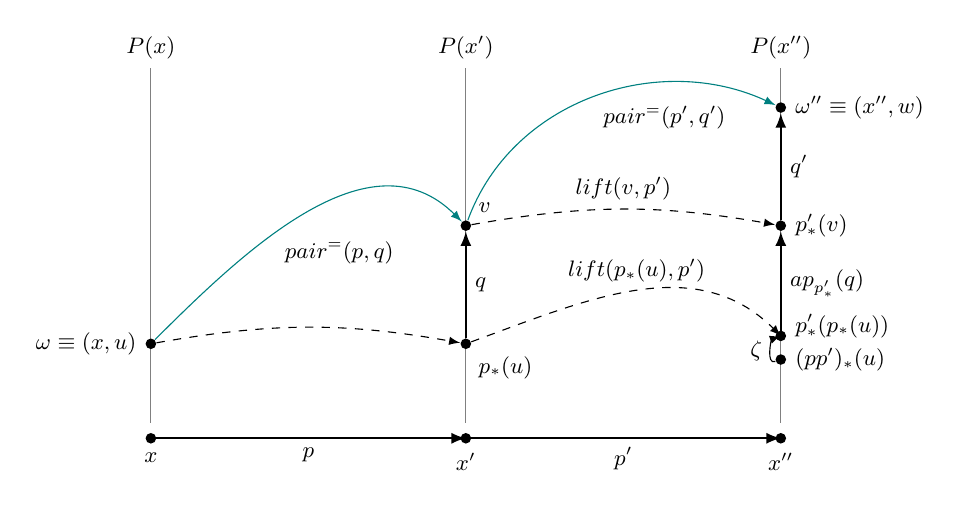
\begin{tikzpicture}[
        >=stealth, 
        scale=1.0,
        font=\small,
        every node/.style={scale=0.9},
        dot/.style={circle, fill, inner sep=1.5pt}
        ]
    
        % Coordinates
        \coordinate (A) at (0,0.3);
        \coordinate (B) at (4,0.3);
        \coordinate (C) at (8,0.3);
    
        % Base Line
        \draw[thick, -latex] (A) -- node[below] {$p$} (B);
        \draw[thick, -latex] (B) -- node[below] {$p'$} (C);
        \node[dot, label=below:$x$] at (A) {};
        \node[dot, label=below:$x'$] at (B) {};
        \node[dot, label=below:$x''$] at (C) {};
    
        % Fibers (visualized as vertical dashed lines)
        \draw[gray] (0,0.5) -- (0,5)
            node[above,black] {$P(x)$};
        \draw[gray] (4,0.5) -- (4,5)
            node[above,black] {$P(x')$};
        \draw[gray] (8,0.5) -- (8,5)
            node[above,black] {$P(x'')$};
    
        % Fiber over x
        \node[dot, label=left:{$\omega\equiv(x,u)$}] (u) at (0,1.5) {};
    
        % Fiber over x'
        \node[dot, label=below right:{$p_*(u)$}] (pu) at (4,1.5) {};
        \node[dot, label=above right:{$v$}] (v) at (4,3.0) {};
        
        % Path q in fiber x'
        \draw[thick,-latex] (pu) -- node[right] {$q$} (v);
    
        % Fiber over x''
        \node[dot, label=right:{$(p\ct p')_*(u)$}] (ppu) at (8,1.3) {};
        \node[circle,
            fill,
            inner sep=1.5pt,
            label={[yshift=4pt]right:{$p'_*(p_*(u))$}}] 
                (pprimeu) at (8,1.6) {};
        \draw[-latex] (ppu) to[out=200,in=200] node[midway, left] {$\zeta$} (8,1.6);
        % Note: visually separating p'*(p*(u)) might be too cluttered, so we treat the coherence \zeta as the bottom anchor point or a tiny loop, but conceptually it starts here.
        
        \node[dot, label=right:{$p'_*(v)$}] (pv) at (8,3.0) {};
        \node[dot, label=right:{$\omega''\equiv(x'',w)$}] (w) at (8,4.5) {};
    
        % Transport arrows (Horizontal)
        \draw[-latex, dashed] (u) to[bend left=10] (pu);
        \draw[-latex, dashed] (pu) to[out=20,in=135] node[above, pos=0.5] {$\fun{lift}(p_*(u),p')$} (8,1.6); % Slight offset to show distinct endpoints
        \draw[-latex, dashed] (v) to[bend left=10] node[above,pos=0.5] {$\fun{lift}(v,p')$} (pv);
    
        % The paths in the third fiber (The Sum)
        
        % 1. The Coherence (approximated as the gap/start)
        % 2. The transported q
        \draw[thick, -latex] (8,1.6) -- node[right] {$\fun{ap}_{p'_*}(q)$} (pv);
        
        % 3. The path q'
        \draw[thick, -latex] (pv) -- node[right] {$q'$} (w);
    
        % Labels for the total paths
        \draw[teal,-latex](u) to[out=45,in=135]
            node[
                pos=0.4,
                below right,
                black] {$\fun{pair}^=(p,q)$} (v);
        \draw[teal,-latex] (v) to[out=70,in=155]
            node[
                midway,
                below right,
                black] {$\fun{pair}^=(p',q')$} (w);
    \end{tikzpicture}
    \]
\end{proof}

\begin{cor}\label{cor:Sigma-pair-inverse}
    Given $p\colon\pi_1(\omega)\eq A\pi_1(\omega')$, we have
    \[
        \bigl(
        \fun{pair}^=(p^{-1},\fun{refl}_{\pi_2(\omega)})
        \bigr)^{-1}
        \eq E
        \fun{pair}^=(p,\fun{refl}_{\pi_2(\omega)}).
    \]
\end{cor}

\begin{proof}
    Even though this can be obtained from part b) of the previous proposition, a proof by path induction is much simpler.

    In the case where $\omega'\equiv\omega$ and $p\equiv\fun{refl}_{\pi_1(\omega)}$ we have
    \begin{align*}
        \lhs&\equiv\bigl(
                \fun{pair}^=(\fun{refl}_{\pi_1(\omega)}^{-1},
                    \fun{refl}_{\pi_2(\omega)})
                \bigr)^{-1}\\
                &\equiv\bigl(
                    \fun{pair}^=(\fun{refl}_{\pi_1(\omega)},
                    \fun{refl}_{\pi_2(\omega)})
                \bigr)^{-1}
                &&\text{; Prop.~\ref{prop:Sigma-pair=-properties}
                    a)}\\
            &\equiv\fun{refl}_\omega^{-1}\\
            &\equiv\fun{refl}_\omega.\\[2mm]
        \rhs&\equiv
                \fun{pair}^=(\fun{refl}_{\pi_1(\omega)}
                ,\fun{refl}_{\pi_2(\omega)})\\
            &\equiv\fun{refl}_\omega.
                &&\text{; Prop.~\ref{prop:Sigma-pair=-properties}
                    a)}\\
    \end{align*}
\end{proof}

\section{The Unit Type}

To apply the framework~\ref{observational-framework} to the unit type $\fun1$, we proceed as in the previous cases.

\textsc{Code family:}
\begin{align*}
    \fun{Code}&\colon\fun1\to\fun1\to\univ\\
    \fun{Code}(x,y)&\defeq\fun1.
\end{align*}

\textsc{Base code:}
For $c\colon\fun{Code}(x,x)$ we specify $c\defeq\fun\star$.

\needspace{2\baselineskip}
\textsc{Encode function:}
\begin{align*}
    \fun{encode}&\colon(x\eq{\fun1}y)\to\fun{Code}(x,y)\\
    \fun{encode}(p)&\defeq\fun{transport}^{C_x}(p,c)
\end{align*}
In particular, for $y\equiv x$ and $p\equiv\fun{refl}_x$, we have
\[
    \fun{encode}(\fun{refl}_x)\equiv c\equiv\fun\star.
\]
Therefore, by induction on $p$, we deduce that
\[
    \fun{encode}(p)\eq{\fun1}\fun\star
\]
and we take the \rhs to define the constant encode function $f\defeq\lambda x,y.\,\lambda p.\,\fun\star$.

\textsc{Decode function:}
Let $g$ denote the backward $\fun{decode}$ map. Then
\[
    g\colon\prod_{x,y\colon\fun1}\fun{Code}(x,y)\to(x\eq{\fun1}y).
\]
To define it we proceed by induction on $x$. It suffices to construct $g(\star)$. The goal becomes a term of type
\[
    \prod_{y\colon\fun1}\fun1 \to (\star\eq{\fun1}y).
\]
Induction on $y$ further reduces the goal to $\fun1 \to (\star\eq{\fun1}\star)$, which is inhabited by the constant function $z\mapsto\fun{refl}_\star$. In particular,
\begin{equation}\label{eq:decode(star)}
    \fun{decode}(\fun\star)\equiv\fun{refl}_{\fun\star}.
\end{equation}

Thus, we have defined $g\colon\prod_{x,y\colon\fun1}\fun1\to(x\eq{\fun1}y)$ as the unique function that satisfies $g(\star,\star,\star) \equiv \fun{refl}_\star$.


\begin{thm}\label{thm:1-equivalence}
    For any\/ $x,y\colon\fun1$, we have\/ $(x\eq{\fun1}y)\simeq\fun1$.
\end{thm}

\begin{proof}
    To verify the homotopies, we need to prove
    \begin{enumerate}[a),font=\upshape]
        \item $f\circ g \sim \id_{\fun1}$.

        This translates into\/ $f(g(x,y,u)) \eq{\fun1} u$ for all\/ $x,y,u\colon\fun1$.
        By the induction principle of\/ $\fun1$, we may set\/ $x,y,u\equiv\star$, which satisfies the goal because\/ $f$ maps every element to\/ $\star$.

        \item $g\circ f \sim \id_{\prod_{x,y\colon\fun1}(x\eq{\fun1}y)}$.

        We must show\/ $g(x,y,f(x,y,p))\eq{x\eq{\fun1}y}p$.
        By path induction, it suffices to check the case\/ $y\equiv x$ and\/ $p\equiv\fun{refl}_x$. The goal becomes
        \[
            g(x,x,f(x,x,\fun{refl}_x))\eq{x\eq{\fun1}x}\fun{refl}_x.
        \]
        By induction on\/ $x$, it is enough to prove\/ $g(\star,\star,f(\star,\star,\fun{refl}_\star))\eq{\star\eq{\fun1}\star}\fun{refl}_\star$. Since\/ $f(\star,\star,\fun{refl}_\star)\equiv\star$, the goal reduces to\/ $g(\star,\star,\star)\eq{\star\eq{\fun1}\star}\fun{refl}_\star$, which holds by the definition of\/ $g$.\qedhere
    \end{enumerate}
\end{proof}

The theorem has the following consequences:

\begin{description}[font=\normalfont\itshape]
    \item[Introduction rule.]
    We define the canonical element inhabiting the identity type of the unit for any two points
    \[
        \fun{triv} \colon x \eq{\fun1} y
    \]
    as\/ $\fun{triv}\defeq\fun{decode}(x,y,\star)$.

    \item[Elimination rule.]
    The dependent eliminator asserts that to define a function out of the identity type, we only need to specify its value on the canonical element.
    \[
        \fun{ind}_{=_{\fun1}}\colon
        \prod_{C\colon(x\eq{\fun1}y)\to\univ}
        C(\fun{triv})\to\prod_{p\colon x\eq{\fun1}y} C(p)
    \]

    \item[Computation rule.]
    When the eliminator is applied to the canonical element\/ $\fun{triv}$, it reduces propositionally\footnote{This is weaker than usual. The equality at the base case is definitional if we accept the\/ $\eta$-rule for the identity type [cf.~\nameref{subsection:eta-rule}].} to the base case\/ $c\colon C(\fun{triv})$.
    \[
        \fun{ind}_{=_{\fun1}}(C,c,\fun{triv})\eq{C(\fun{triv})}c.
    \]

    \item[Uniqueness rule.]
    This rule asserts that the type is contractible (a singleton); any inhabitant\/ $p$ is path-equal to the canonical element.
    \[
        \fun{uniq}_{=_{\fun1}}\colon
        \prod_{p\colon x\eq{\fun1}y}p
            \eq{x\eq{\fun1}y}\fun{triv}.
    \]
\end{description}

To derive the elimination rule, we use Theorem~\ref{thm:1-equivalence}, which gives us a homotopy:
\[
    \varepsilon_p\colon
        \fun{decode}(x,y,\fun{encode}(x,y,p))\eq{\fun1}p
\]
for every path\/ $p\colon x\eq{\fun1}y$. Since, by definition, $\fun{encode}(x,y,p)\equiv\fun\star$, the homotopy simplifies:
\[
    \fun{decode}(x,y,\fun{encode}(x,y,p))
        \equiv\fun{decode}(x,y,\star)\equiv\fun{triv},
\]
and so
\[
    \varepsilon_p \colon \fun{triv}\eq{x\eq{\fun1}y}p.
\]
Now, given\/ $C\colon(x\eq{\fun1}y)\to\univ$ and\/ $c\colon C(\fun{triv})$, we want to construct\/ $f(p)\colon C(p)$.

We define
\[
    \fun{ind}_{=_{\fun1}}(C,c,p)
        \defeq\fun{transport}^C(\varepsilon_p,c).
\]
In the case\/ $p\equiv\fun{triv}$, we have:
\begin{equation}\label{eq:eta-rule-dependent}
    \varepsilon_{\fun{triv}}
        \eq{x\eq{\fun1}y}\fun{refl}_{\fun{triv}}.
\end{equation}
Therefore:
\begin{equation}\label{eq:definitional-base-case}
    \fun{ind}_{=_{\fun1}}(C,c,\fun{triv})
        \eq{C(\fun{triv})}
        \fun{transport}^C(\fun{refl}_{\fun{triv}},c)
        \equiv c.
\end{equation}

The Uniqueness rule is derived by taking the symmetry (inverse) of $\varepsilon_p$:
    \[
        \fun{uniq}_{=_{\fun1}}(p) \defeq \varepsilon_p^{-1}.
    \]

\subsection*{The $\eta$-rule for the Identity of\/ $\fun1$}
\label{subsection:eta-rule}

The\/ $\eta$-rule asserts that every inhabitant of the identity type of the unit is definitionally equal to reflexivity, namely
\begin{equation*}
    p\equiv\fun{refl}_{\fun\star}
    \qquad(\text{for every } p\colon x\eq{\fun1}y).
\end{equation*}
Since the\/ $\eta$-rule for the Identity of\/ $\fun1$ is structurally impossible to state (as a general rule for arbitrary\/ $x,y$) without first assuming the\/ $\eta$-rule for\/ $\fun1$, this requires the\/ $\eta$-rule for the unit type.

\textbf{Extended framework.} For the unit type identity, we have
\begin{align*}
    \fun{inv}&\colon\fun{Code}(x,y)\to\fun{Code}(y,x)\\
    \fun{inv}(u)&\defeq u
\intertext{and}
    \ect&\colon\fun{Code}(x,y)\to\fun{Code}(y,z)
        \to\fun{Code}(x,z)\\
    u\ect v&\defeq v.
\end{align*}
The unit laws follow directly from the definitions above, namely
\begin{align*}
    \fun{inv}(c)&\equiv c\\
    c\ect u&\equiv u.
\end{align*}

\begin{prop}
    Given $x,y,z\colon\fun1$, and $p\colon x\eq{\fun1}y$ and $q\colon y\eq{\fun1}z$, we have
    \begin{enumerate}[a),font=\upshape]
        \item $\fun{decode}(x,x,\fun\star)\eq{x\eq{\fun1}x}\fun{refl}_x$
        
        \item $\fun{decode}(y,x,u)\eq{y\eq{\fun1}x}\fun{decode}(x,y,u)^{-1}$
        
        \item $\fun{decode}(x,z,u\ect v)\eq{x\eq{\fun1}z}\fun{decode}(x,y,u)\ct\fun{decode}(y,z,v)$
    \end{enumerate}
\end{prop}

\begin{proof}
    This is a direct consequence of Theorem~\ref{thm:extended-framework}.
    %
    
\end{proof}

\section{Function Extensionality Axiom}

In this section we address the question of the identity type for dependent (and non-dependent) functions. To establish the context, let\/ $A\colon\univ$ be a type and\/ $B\colon A\to\univ$ a type family. To analyze the identity in the section space\footnote{Consisting of all dependent functions\/ $s\colon A\to E$, where\/ $E$ is the total space\/ $\sum_{x\colon A}B(x)$, such that\/ $\pi_1(s(x))\eq A x$ for all\/ $x\colon A$.}
\[
    \Gamma\defeq\prod_{x\colon A}B(x)
\]
we apply the framework~\ref{observational-framework}.

\textsc{Code family:}
\begin{align*}
    \fun{Code}&\colon\Gamma\to\Gamma\to\univ\\
    \fun{Code}(f,g)&\defeq\prod_{x\colon A} f(x)\eq{B(x)}g(x).
\end{align*}

\textsc{Base code:} For the reflexive case, we define the term\/ $c\colon\fun{Code}(f,f)$ pointwise by reflexivity:
\[
    c \defeq \lambda x\colon A.\, \fun{refl}_{f(x)}.
\]

\textsc{Encode function:}
\begin{align*}
    \fun{encode}&\colon(f\eq\Gamma g)\to\fun{Code}(f,g)\\
    \fun{encode}(p)&\defeq\fun{transport}^{C_f}(p,c).
\end{align*}
Since\/ $C_f\defeq\fun{Code}(f,{}\cdot{})$, we can define the local family at a point\/ $x\colon A$ as
\[
    C_{f,x}\defeq\lambda h\colon\Gamma.\, f(x)\eq{B(x)}h(x).
\]
In particular, in the case where\/ $g\equiv f$ and\/ $p\equiv\fun{refl}_f$, we have
\begin{align*}
    \fun{encode}(\fun{refl}_f)(x)
        &\equiv\fun{transport}^{C_f}(\fun{refl}_f,c)(x)\\
        &\equiv c(x)\\
        &\equiv\fun{refl}_{f(x)}\\
        &\equiv\fun{transport}^{C_{f,x}}
            (\fun{refl}_f,\fun{refl}_{f(x)}).
\end{align*}
Hence, path induction implies
\[
    \fun{encode}(p)(x)\eq{C_{f,x}(g)}
        \fun{transport}^{C_{f,x}}(p,\fun{refl}_{f(x)}),
\]
for $p\colon f\eq\Gamma g$ and $x\colon A$.
We take the \rhs to define the standard name for the encode function \textsl{homotopy application\/}:
\begin{equation}\label{eq:homotopy-application}
    \begin{aligned}
        \fun{happly}&\colon(f\eq\Gamma g)\to\fun{Code}(f,g)\\
        \fun{happly}(p)&\defeq \lambda x\colon A.\,
                \fun{transport}^{C_{f,x}}(p,\fun{refl}_{f(x)})
    \end{aligned}
\end{equation}
and introduce the following

\textbf{Axiom.} [Function Extensionality] The homotopy application function \eqref{eq:homotopy-application} is an equivalence.\footnote{We will see in later chapters that this axiom follows both from univalence and from the interval type.}

Thus, the axiom asserts that\/ $\fun{happly}$ has a quasi-inverse
\begin{align*}
    \fun{funext}&\colon\fun{Code}(f,g)\to(f\eq\Gamma g),
\end{align*}
which, by definition, satisfies the following homotopies for any path\/ $p\colon f\eq\Gamma g$ and any pointwise homotopy\/ $\alpha\colon\fun{Code}(f,g)$:
\begin{align*}
    \fun{funext}(\fun{happly}(p))
        &\eq{f\eq\Gamma g} p\\
    \fun{happly}(\fun{funext}(\alpha))
        &\eq{\fun{Code}(f,g)}\alpha.
\end{align*}

\begin{rem}
    The $\fun{funext}$ function acts as the \textit{introduction rule} (or constructor) for the identity type of dependent functions, as it generates paths from homotopies. Consequently, the fact that it is an equivalence justifies the \textit{induction principle}: to prove a property for all paths, it suffices to check those constructed by $\fun{funext}$. More generally, every $\fun{decode}$ function acts as an introduction rule, while the $\fun{encode}$ functions can be seen as \textit{elimination rules}: they extract structural features from the path.
\end{rem}

\textbf{Extended framework.} To apply the framework~\ref{extended-framework}, we define
\begin{align*}
    \fun{inv}&\colon\fun{Code}(f,g)\to\fun{Code}(g,f)\\
    \fun{inv}(u)&\defeq\lambda x\colon A.\,u(x)^{-1}
\intertext{and}
    \ect&\colon\fun{Code}(f,g)\to\fun{Code}(g,h)
        \to\fun{Code}(f,h)\\
    u\ect v&\defeq\lambda x\colon A.\,u(x)\ct v(x).
\end{align*}
The unit laws follow immediately from the definitional properties of path inversion and concatenation applied pointwise:
\begin{align*}
    \fun{inv}(c)&\equiv\lambda x.\,\fun{refl}_{f(x)}^{-1}\\
        &\equiv\lambda x.\,\fun{refl}_{f(x)}\\
        &\equiv c,
\intertext{and}
    c\ect u&\equiv\lambda x.\,c(x)\ect u(x)\\
        &\equiv\lambda x.\,\fun{refl}_{f(x)}\ct u(x)\\
        &\equiv\lambda x.\, u(x)\\
        &\equiv u.
\end{align*}

\begin{prop}
    Let\/ $A$,\/ $B$, and\/ $\Gamma$ be as above. If\/ $f, g\colon\Gamma$, then
    \begin{enumerate}[a),font=\upshape]
        \item $\fun{funext}(f,f,\lambda x.\,\fun{refl}_{f(x)})\eq{f\eq\Gamma f}\fun{refl}_f$

        \item For\/ $u\colon\prod_{x\colon A}f(x)\eq{B(x)}g(x)$, we have
        \[
            \fun{funext}(g,f,\lambda x.\,u(x)^{-1})\eq{g\eq\Gamma f}
            \fun{funext}(f,g,u)^{-1}
        \]

        \item Given\/ $h\colon\Gamma$ and\/ $v\colon\prod_{x\colon A}g(x)\eq{B(x)}h(x)$, we have
        \[
            \fun{funext}(f,h,u\ect v)\eq{f\eq\Gamma h}\fun{funext}(f,g,u)\ct\fun{funext}(g,h,v)
        \]
    \end{enumerate}
\end{prop}

\begin{proof}
    This is an immediate consequence of Theorem~\ref{thm:extended-framework}.
\end{proof}

\subsection*{Non-dependent Functions}

The special case where $B\colon A\to\univ$ is constant refers to the non-dependent function type: $\Gamma\equiv A\to B$. Here the general case computes as follows, for $f,g\colon A\to B$ and $p\colon f\eq{A\to B}g$,
\begin{align*}
    C_{f,x}&\defeq\lambda g.\,f(x)\eq Bg(x)\\
    \fun{happly}(p)&\defeq\lambda x.\,
                \fun{transport}^{C_{f,x}}(p,\fun{refl}_{f(x)})\\
        \fun{funext}&\colon\fun{Code}(f,g)
            \to(f\eq{A\to B}g).
\end{align*}

\subsection*{Transport Decomposition}\label{subs:transport-decomposition}

\paragraph{Non-dependent case.} Let\/ $X\colon\univ$ be a type and\/ $A,B\colon X\to\univ$ be type families. Let\/ $A\to B\colon X\to\univ$ denote (by abuse of notation) the type family
\[
    (A\to B)(x)\defeq A(x)\to B(x).
\]
Given a path\/ $p\colon x\eq X y$ and a function\/ $f\colon (A\to B)(x)$, we have the following diagram:
\begin{equation}\label{tik-constant-transport-composition}
    \begin{tikzcd}[column sep=2.5cm]
        A(x) 
            \arrow[r, "f"] 
            \arrow[d, "{\fun{transport}^A(p)}"'] 
        & B(x) 
            \arrow[d, "{\fun{transport}^B(p)}"] 
        \\
        A(y) 
            \arrow[r, "{\fun{transport}^{A\to B}(p, f)}"'] 
        & B(y)
    \end{tikzcd}
\end{equation}

\begin{prop}
    The diagram~\eqref{tik-constant-transport-composition} propositionally commutes in the function type\/ $A(x)\to B(y)$. In particular,
    \[
        \fun{transport}^{A\to B}(p, f) \eq{}
            \fun{transport}^B(p) \circ f \circ \fun{transport}^A(p^{-1}).
    \]
\end{prop}

\begin{proof}
    First, observe that the diagram is well-typed because
    \[
        \fun{transport}^{A\to B}(p,f)\colon (A\to B)(y) \equiv A(y)\to B(y).
    \]
    To prove the commutativity, by path induction, it suffices to consider the case\/ $y\equiv x$ and\/ $p\equiv\fun{refl}_x$. In this case, we obtain the square
    \[
        \begin{tikzcd}[column sep=2.5cm]
            A(x) 
                \arrow[r, "f"] 
                \arrow[d, "{\fun{transport}^A(\fun{refl}_x)}"'] 
            & B(x) 
                \arrow[d, "{\fun{transport}^B(\fun{refl}_x)}"] 
            \\
            A(x) 
                \arrow[r, "{\fun{transport}^{A\to B}(\fun{refl}_x, f)}"'] 
            & B(x)
        \end{tikzcd}
    \]
    which trivially (and definitionally) commutes because all transports of reflexivity reduce to the identity function.
\end{proof}

\paragraph{Dependent case.} To generalize the non-dependent case, we have to consider the situation where
\begin{align*}
    B&\colon\prod_{x\colon X}A(x)\to\univ.
\intertext{What we had in the non-dependent context becomes}
    \Pi_AB&\colon X\to\univ\\
    \Pi_AB(x)&\defeq\prod_{u\colon A(x)}B(x,u)\\
    f&\colon\Pi_AB(x)
\intertext{Introduce}
    \Sigma_XA&\defeq\sum_{x\colon X}A(x)
        &&\text{(total space)}\\
    \hat B&\colon\Sigma_XA\to\univ
        &&\text{(uncurried $B$)}\\
    \hat{B}(\omega)&\defeq B(\pi_1(\omega),\pi_2(\omega))
        &&\text{(induction principle)}
\end{align*}

\begin{thm}\label{thm:dependent-transport-decomp}
    Given\/ $x,y\colon X$, a path\/ $p\colon x\eq Xy$, and a function\/ $f\colon \Pi_A B(x)$, let\/ $u\colon A(x)$. Define
    \begin{alignat*}2
        p_*&\defeq\fun{transport}^A(p),
        &\quad\gamma&\defeq\fun{pair}^=(p,\fun{refl}_{p_*(u)})
            \colon(x,u)\eq{\Sigma_XA}(y,p_*(u)).
    \end{alignat*}
    Then the following diagram of elements commutes propositionally:
    \[
        \begin{tikzcd}[column sep=huge, row sep=large]
            u
                \arrow[r,mapsto,"p_*"]
                \arrow[d,mapsto,"f"']
            &p_*(u)
                \arrow[d,
                    mapsto,
                    "{\fun{transport}^{\Pi_A B}(p,f)}"] 
        \\
            f(u)
                \arrow[r,mapsto,"\fun{transport}^{\hat B}(\gamma)"']
            &\bigl(\fun{transport}^{\Pi_A B}(p,f)\bigr)
                (p_*(u))
        \end{tikzcd}
    \]
    Explicitly, we have the equality
    \[
        \fun{transport}^{\hat B}(\gamma,f(u))
        \eq{B(y,p_*(u))}
        \bigl(\fun{transport}^{\Pi_A B}(p,f)\bigr)(p_*(u)).
    \]
\end{thm}

\begin{proof}${}$
    \begin{description}[font=\normalfont\scshape]
        \item[Type verification.] 
        Note that, since $u\colon A(x)$, $f(u)\in B(x,u)$. Hence,
        \[
            \fun{transport}^{\hat B}(\gamma)
                \colon B(x,u)\to B(y,p_*(u))
        \]
        and
        \[
            \lhs\equiv\fun{transport}^{\hat B}(\gamma,f(u))
                \colon B(y,p_*(u)).
        \]
        Since
        \begin{align*}
            &\fun{transport}^{\Pi_AB}(p)
                \colon\Pi_A(B)(x)\to\Pi_AB(y),
        \intertext{we obtain,}
            &\fun{transport}^{\Pi_AB}(p,f)\colon\Pi_AB(y),
        \intertext{and so}
            &\rhs\equiv\bigl(\fun{transport}^{\Pi_AB}(p,f)\bigr)(p_*(u))
                \colon B(y,p_*(u)).
        \end{align*}
        Therefore, both compositions compute to the same type $B(y,p_*(u))$.
        \item[Inhabitation.] By path induction, it suffices to consider the case $y\equiv x$ and $p\equiv\fun{refl}_x$. In that case, we deduce that $\gamma\equiv\fun{refl}_{(x,u)}$. Therefore,
        \begin{align*}
            \lhs&\equiv\fun{transport}^{\hat B}
                (\fun{refl}_{(x,u)},f(u))\\
                &\equiv f(u)
        \intertext{and}
            \rhs&\equiv\bigl(\fun{transport}^{\Pi_A B}
                (\fun{refl}_x,f)\bigr)(u)\\
                &\equiv f(u),
        \end{align*}
        which shows that $\lhs\equiv\rhs$.
    \end{description}
%
    
\end{proof}

\begin{rem}
    The previous theorem is to $\Pi$-types what Theorem~\ref{thm:composite-transport} is to $\Sigma$-types. To better visualize the analogy, let us rewrite the equality of Theorem~\ref{thm:composite-transport} using the path $\gamma$ in the total space
    \begin{align*}
        \explain[\text{transport }(u,z)\text{ along }p]
            {\fun{transport}^{\Sigma_AB}(p)(u,z)}
        &\eq{\Sigma_AB(y)}
            \bigl(
            \explain[\text{transport }u]{p_*(u)},
            \explain[\text{transport }z\text{ along }\gamma]
            {\fun{transport}^B(\gamma)(z)}
        \bigr)\\
    \explain[\text{transport }f(u)\text{ along }\gamma]
        {\fun{transport}^{\hat B}(\gamma,f(u))}
        &\eq{B(y,p_*(u))}
        \bigl(
        \explain[\text{transport }f\text{ along }p]
        {\fun{transport}^{\Pi_A B}(p,f)}
        \bigr)(p_*(u)).
    \end{align*}
    In words, we have
    \begin{align*}
        \text{transport a dependent pair}
            &= \text{pair the transports}\\
        \text{transport an evaluation}
            &= \text{evaluate the transport},
    \end{align*}
    Meaning that, in the first case, transport commutes with dependent pairing, while in the second it commutes with function application.
\end{rem}

\begin{cor}\label{cor:dependent-transport-decomp}
    With the precedent notation, for $v\colon A(y)$ we have
    \[
    \fun{transport}^{\Pi_AB}(p,f)(v)
    \eq{B(y,v)}
    \fun{transport}^{\hat B}
    \bigl(
        (
            \delta^{-1},
        f((p^{-1})_*(v))
    \bigr),
    \]
    where $\delta\defeq\fun{pair}^=(p^{-1},\fun{refl}_{(p^{-1})_*(v)})$.
\end{cor}

\begin{proof}
    Even though this can be derived from the theorem, it is much simpler to use path induction and verify the definitionally equality in the case $y\equiv x$ and $p\equiv\fun{refl}_x$. In fact, in that case we obtain
    \begin{align*}
        \lhs&\equiv
            \fun{transport}^{\Pi_AB}(\fun{refl}_x,f)(v)\\
            &\equiv f(v),\\
        \delta&\equiv\fun{pair}^=(\fun{refl}_x
            ,\fun{refl}_{(\fun{refl}_x)_*(v)})
                &&;\ \fun{refl}_x^{-1}\equiv\fun{refl}_x\\
            &\equiv\fun{refl}_{(\fun{refl}_x)_*(v)}\\
            &\equiv\fun{refl}_v,\\
        \rhs
        &\equiv
            \fun{transport}^{\hat B}
            \bigl(
                (
                    \fun{refl}_v,
                    f((\fun{refl}_x)_*(v))
            \bigr)
            &&;\ \fun{refl}_x^{-1}\equiv\fun{refl}_x\\
        &\equiv f((\fun{refl}_x)_*(v))\\
        &\equiv f(v).
    \end{align*}
\end{proof}

\begin{cor}
    With the precedent notation, for\/ $v\colon A(y)$ we have
    \[
        \fun{transport}^{\Pi_AB}(p,f)(v)
        \eq{B(y,v)}
        \fun{transport}^{\hat B}
        \bigl(
            \delta^{-1},
            f((p^{-1})_*(v))
        \bigr),
    \]
    where\/ $\delta\defeq\fun{pair}^=(p^{-1},\fun{refl}_{(p^{-1})_*(v)})$.
\end{cor}

\begin{proof}
    Even though this can be derived from the theorem, it is simpler to use path induction and verify the definitional equality in the case\/ $y\equiv x$ and\/ $p\equiv\fun{refl}_x$.
    In that case, we obtain
    \begin{align*}
        \lhs&\equiv
            \fun{transport}^{\Pi_AB}(\fun{refl}_x,f)(v)\\
            &\equiv f(v).
    \intertext{For the right-hand side, since\/ $p^{-1}\equiv\fun{refl}_x$, we have}
        \delta&\equiv\fun{pair}^=(\fun{refl}_x
            ,\fun{refl}_{(\fun{refl}_x)_*(v)})\\
            &\equiv\fun{pair}^=(\fun{refl}_x, \fun{refl}_v)\\
            &\equiv\fun{refl}_{(x,v)}.
    \intertext{Thus,\/ $\delta^{-1}\equiv\fun{refl}_{(x,v)}$ and}
        \rhs
        &\equiv
            \fun{transport}^{\hat B}
            \bigl(
                \fun{refl}_{(x,v)},
                f((\fun{refl}_x)_*(v))
            \bigr)\\
        &\equiv f((\fun{refl}_x)_*(v)\\
        &\equiv f(v).
    \end{align*}
    This shows that\/ $\lhs\equiv\rhs$.
\end{proof}

\begin{lem}\label{lem:non-dependent-i-j-paths}
    Let\/ $A\colon X\to\univ$ be a type family and\/ $p\colon x\eq Xy$ a path in~$X$. Then, given a second type family\/ $B\colon X\to\univ$ and a non-dependent function\/ $f\colon A(x)\to B(x)$, for any\/ $u\colon A(x)$ there are two paths
    \begin{equation}\label{eq:non-dependent-i-j-paths}
        \begin{aligned}
            i(p,u)&\colon p_*(f)(p_*(u))
                \eq{B(y)}p_*\bigl(f(p^{-1}_*(p_*(u)))\bigr),\\
            j(p,u)&\colon p_*\bigl(f(p^{-1}_*(p_*(u)))\bigr)
                \eq{B(y)}p_*(f(u)),
        \end{aligned}
    \end{equation}
    where we use the abbreviations:
    \begin{equation}\label{eq:non-dependent-p*-meanings}
        \begin{aligned}
            p_*(f)&\defeq\fun{transport}^{A\to B}(p,f),\\
            p_*(f(u))&\defeq\fun{transport}^B(p,f(u)),\\
            p_*(u)&\defeq\fun{transport}^A(p,u).
        \end{aligned}
    \end{equation}
\end{lem}

\begin{proof}
    Define the motive
    \begin{align*}
        P&\colon\prod_{y\colon X}(x\eq Xy)\to\univ\\
        P(y,p)&\defeq \prod_{u\colon A(x)}
            \fun{Eq}_i(y,p,u) \times \fun{Eq}_j(y,p,u),
    \end{align*}
    where $\fun{Eq}_i$ and $\fun{Eq}_j$ correspond to the identity types corresponding to $i(p,u)$ and $j(p,u)$.
    
    By based path induction, it suffices to construct an inhabitant of $P(x,\fun{refl}_x)$.
    In this case, given $u\colon A(x)$, both equalities reduce to $f(u)\eq{B(x)}f(u)$. Hence,
    \[
        \lambda u.\,(\fun{refl}_{f(u)},\,\fun{refl}_{f(u)})
            \colon P(x,\fun{refl}_x).
    \]
\end{proof}

\begin{thm}\label{thm:function-equality-equivalence}
    Let\/ $A\colon X\to\univ$ be a type family and\/ $p\colon x\eq Xy$ a path in $X$. Then, given a second type family $B\colon X\to\univ$ and two functions\/ $f\colon A(x)\to B(x)$ and\/ $g\colon A(y)\to B(y)$, there is an equivalence
    \begin{align*}
        \bigl(p_*(f)\eq{A(y)\to B(y)}g\bigr)
            &\simeq\prod_{u\colon A(x)}p_*(f(u))\eq{B(y)}g(p_*(u)).
    \end{align*}
    Moreover, if\/ $q\colon p_*(f)\eq{A\to B}g$ corresponds under this equivalence to\/ $\hat q$, then for any\/ $u\colon A(x)$, the path
    \[
        \fun{happly}(q,p_*(u))
            \colon p_*(f)(p_*(u))\eq{B(y)}g(p_*(u))
    \]
    satisfies
    \[
        \fun{happly}(q,p_*(u))
        \eq{B(y)}
        i(p,u)\ct j(p,u)\ct\hat q(u),
    \]
    where\/ $i(p,u)$ and\/ $j(p,u)$ are the paths given by\/ \eqref{eq:non-dependent-i-j-paths}.
\end{thm}

\begin{proof}
    To define the motive
    \[
        P\colon\prod_{y\colon X}(x\eq Xy)\to\univ,
    \]
    we proceed as follows:
    \begin{enumerate}[-]
        \item For $y\colon X$ and $p\colon x\eq Xy$, let
        \begin{align*}
            \fun L(y,p,g)
                &\defeq p_*(f)\eq{A(y)\to B(y)}g,\\
            \fun R(y,p,g)
                &\defeq\prod_{u\colon A(x)}
                p_*(f(u))\eq{B(y)} g(p_*(u)).
        \end{align*}

        \item Then define
        \[
            P(y,p)\defeq\prod_{g\colon A(y)\to B(y)}
                \;\sum_{e\colon \fun L\simeq\fun R}
                \fun E(y,p,g,e),
        \]
        where
        \[
            \fun E(y,p,g,e)\defeq\!\!\!
                \prod_{q\colon\fun L(y,p,g)}
                \,\prod_{u\colon A(x)}
                    \!\!\fun{happly}(q,p_*(u))
                    \eq{B(y)}
                    i(p,u)\ct j(p, u)\ct e(q)(u),
        \]
        and $i(p,u)$ and $j(p,u)$ are the paths defined in \eqref{eq:non-dependent-i-j-paths}. The following diagram shows that $\fun E$ is well defined:
        \[
            \begin{tikzcd}[column sep=4em, row sep=3em]
                p_*(f)(p_*(u))
                        \arrow[r,"{\fun{happly}(q, p_*(u))}"]
                        \arrow[d,"{i(p,u)}"']
                    &g(p_*(u))\\
                {p_*\bigl(f((p^{-1})_*(p_*(u)))\bigr)}
                        \arrow[r,"{j(p,u)}"']
                    &{p_*(f(u))}
                        \arrow[u,"e(q)(u)"']
            \end{tikzcd}
        \]
    \end{enumerate}
    By based path induction, i.e., by equation \eqref{eq:ind'=A} applied to $P(y,p)$, we have to construct an inhabitant for the case where $y\equiv x$ and $p\equiv\fun{refl}_x$. In this case:
    \begin{enumerate}[-]
        \item $p_*\equiv\id$, $\fun L(x,\fun{refl}_x,g)\equiv f\eq{A(x)\to B(x)}g$, and $\fun R(x,\fun{refl}_x,g)\equiv f\sim g$.

        \item $i(\fun{refl}_x,u)\equiv\fun{refl}_{f(u)}$ and $j(\fun{refl}_x,u)\equiv\fun{refl}_{f(u)}$.

        \item We choose $e\defeq\fun{happly}$, which is an equivalence by the Function Extensionality Axiom.
        The type $\fun E(x,\fun{refl}_x,g,\fun{happly})$ requires us to verify that for every $q\colon f\eq{A(x)\to B(x)}g$ and $u\colon A(x)$,
        \[
            \fun{happly}(q,u)
            \eq{B(x)}
            \fun{refl}_{f(u)}
                \ct \fun{refl}_{f(u)}
                \ct\fun{happly}(q,u).
        \]
        But this is inhabited by $\fun{refl}_{\fun{happly}(q,u)}$.
    \end{enumerate}
    Thus, the map
    \[
        g\mapsto(\fun{happly}
        ,\lambda q.\,\lambda u.\,\fun{refl}_{\fun{happly}(q,u)})
    \]
    inhabits $P(x,\fun{refl}_x)$, which completes the proof.
\end{proof}

What follows is a generalization of Lemma~\ref{lem:non-dependent-i-j-paths} and Theorem~\ref{thm:function-equality-equivalence} for dependent functions. The notation is the one introduced in the Dependent case of section \nameref{subs:transport-decomposition}.

\begin{lem}\label{lem:dependent-i-j-path}
    Let $A\colon X\to\univ$ be a type family and $p\colon x\eq Xy$ a path in~$X$. Then, given a second type family $B\colon\prod_{x\colon X}A(x)\to\univ$ and a dependent function $f\colon\Pi_AB(x)$, we have
            \begin{align*}
                i(p,u)&\colon p_*(f)(p_*(u))
                    \eq{B(y,p_*(u))}\Phi((p^{-1})_*(p_*(u)))\\
                j(p,u)&\colon \Phi((p^{-1})_*(p_*(u)))
                    \eq{B(y,p_*(u))}\fun{Tr}(p,f,u),
            \end{align*}
            with
            \begin{align*}
                \Phi(w)&\defeq
                    \fun{transport}^{\hat B}
                    \bigl(\fun{pair}^=
                        (p^{-1},\fun{refl}_w)^{-1},f(w)
                    \bigr)\\
                \fun{Tr}(p,f,u)&\defeq
                    \fun{transport}^{\hat B}
                    \bigl(
                        \fun{pair}^=(p,\fun{refl}_{p_*(u)}),
                        f(u)
                    \bigr).
            \end{align*}
\end{lem}

\begin{proof}
    To proceed with type verification, observe that\footnote{See the notation used in Theorem~\ref{thm:dependent-transport-decomp}.}
    \begin{alignat*}6
        u&\colon A(x),&\quad p_*(u)&\colon A(y),
            &\quad w\equiv(p^{-1})_*(p_*(u))&\colon A(x).
    \end{alignat*}
    Thus,
    \begin{alignat*}4
        \fun{pair}^=(p^{-1},\fun{refl}_w)^{-1}
                &\colon(x,u)\eq{\Sigma_XA}(y,p_*(u)),
                &\quad f(w)&\colon B(x,u),\\
        \Phi(w)&\colon B(y,p_*(u)),
            &\quad\fun{Tr}(p,f,u)&\colon B(y,p_*(u)).
    \end{alignat*}
    Then all expressions are correctly typed.
    
    To construct the witnesses $i(p,u)$ and $j(p,u)$, define the motive
    \begin{align*}
        P&\colon\prod_{y\colon X}(x\eq Xy)\to\univ\\
        P(y,p)&\defeq\prod_{u\colon A(x)}
            \fun{Eq}_i(y,p,u)\times\fun{Eq}_j(y,p,u),
    \end{align*}
    where $\fun{Eq}_i$ and $\fun{Eq}_j$ are the types of $i(p,u)$ and $j(p,u)$.

    By based path induction, to show that $P(y,p)$ is inhabited it suffices to construct a witness of $P(x,\fun{refl}_x)$. In this case:
    \begin{enumerate}[-]
        \item $p$ and $p^{-1}$ reduce definitionally to $\fun{refl}_x$.
        
        \item Since the transport operations $p_*$ reduce to identity functions, $p_*(u) \equiv u$ and $p_*(f) \equiv f$.
        
        \item The fiber coordinate $w\defeq(p^{-1})_*(p_*(u))$ reduces definitionally to $u$.
        
        \item $\Phi(w)$ becomes $f(u)$.

        \item $\fun{Tr}(\fun{refl}_x,f,u)$ becomes:
        \[
            \fun{transport}^{\hat B}
            \bigl(
                \fun{pair}^=(\fun{refl}_x,\fun{refl}_u),
                f(u)
            \bigr),
        \]
        which is definitionally equal to $f(u)$.
    \end{enumerate}

    Consequently, for any $u\colon A(x)$, the goals become:
    \begin{align*}
        i(\fun{refl}_x, u) &\colon f(u) \eq{B(x,u)} f(u),\\
        j(\fun{refl}_x, u) &\colon f(u) \eq{B(x,u)} f(u).
    \end{align*}
    These are clearly inhabited by $\fun{refl}_{f(u)}$.
    Thus, the term
    \[
        \lambda u.\,(\fun{refl}_{f(u)},\, \fun{refl}_{f(u)})
    \]
    witnesses $P(x,\fun{refl}_x)$, completing the proof.

\end{proof}

\begin{thm}
    Given two families\/ $A\colon X\to\univ$ and\/ $B\colon\prod_{x\colon X}A(x)\to\univ$, a path\/ $p\colon x\eq Xy$, and functions\/ $f\colon\Pi_AB(x)$ and\/ $g\colon\Pi_AB(y)$, there is an equivalence
    \[
        \bigl(p_*(f)\eq{\Pi_AB(y)}g\bigr)
        \simeq
        \prod_{u\colon A(x)}
        \fun{Tr}(p,f,u)
        \eq{B(y,p_*(u))}
        g(p_*(u)),
    \]
    where
    \[
        \fun{Tr}(p,f,u)\defeq
            \fun{transport}^{\hat B}
            \bigl(
                \fun{pair}^=(p,\fun{refl}_{p_*(u)}),
                f(u)
            \bigr)
    \]
    Moreover, if\/ $q\colon p_*(f)\eq{\Pi_AB(y)}g$ corresponds under this equivalence to\/ $\hat q$, then for any\/ $u\colon A(x)$, the path
    \[
        \fun{happly}(q,p_*(u))
        \colon p_*(f)(p_*(u))\eq{B(y,p_*(u))}g(p_*(u))
    \]
    is equal to the concatenated path
    \[
        i(p,u)\ct j(p,u)\ct\hat q(u),
    \]
    where\/ $i(p,u)$ and $j(p,u)$ are the paths given by\/ {\upshape Lemma~\ref{lem:dependent-i-j-path}}. In a diagram
    \[
        \begin{tikzcd}[column sep=7em, row sep=3em]
            p_*(f)(p_*(u))
                    \arrow[r,"{\fun{happly}(q, p_*(u))}"]
                    \arrow[d,"{i(p,u)}"']
                &g(p_*(u))\\
            \Phi(w)
                    \arrow[r,"{j(p,u)}"']
            &\fun{Tr}(p,f,u)
                    \arrow[u,"\hat q(u)"']
        \end{tikzcd}
    \]
\end{thm}

\begin{proof}
    To define the motive
    \[
        P\colon\prod_{y\colon X}(x\eq Xy)\to\univ
    \]
    \needspace{2\baselineskip}
    proceed as follows:
    \begin{enumerate}[-]
        \item For $y\colon X$ and $p\colon x\eq Xy$, let
        \begin{align*}
            \fun L(y,p,g)
                &\defeq p_*(f)\eq{\Pi_AB(y)}g,\\
            \fun R(y,p,g)
                &\defeq\prod_{u\colon A(x)}
                \fun{Tr}(p,f,u) \eq{B(y,p_*(u))} g(p_*(u)).
        \end{align*}

        \item Then define
        \[
            P(y,p)\defeq\prod_{g\colon\Pi_AB(y)}
                \;\sum_{e\colon \fun L\simeq\fun R}
                \fun E(y,p,g,e),
        \]
        where
        \[
            \fun E(y,p,g,e)\defeq\!\!\!
                \prod_{q\colon\fun L(y,p,g)}
                \,\prod_{u\colon A(x)}
                    \!\!\fun{happly}(q,p_*(u))
                    \eq{B(y,p_*(u))}
                    \delta(p,u)\ct e(q)(u),
        \]
        with $\delta(p,u)\defeq i(p,u)\ct j(p,u)$.
    \end{enumerate}
    By based path induction, it suffices to specify an inhabitant for the case where $y\equiv x$ and $p\equiv\fun{refl}_x$. In this case:
    \begin{enumerate}[-]
        \item $\fun L(x,\fun{refl}_x,g)\equiv f\eq{\Pi_AB(x)}g$,  $\fun{Tr}(\fun{refl}_x,f,u)\equiv f(u)$, $\fun R(x,\fun{refl}_x,g)\equiv f\sim g$.

        \item $i(\fun{refl}_x,u)$ and $j(\fun{refl}_x,u)$ reduce to $\fun{refl}_{f(u)}$.

        \item Take $e\defeq\fun{happly}$. The type $\fun E(x,\fun{refl}_x,g,\fun{happly})$ requires us to verify that for every $q\colon f\eq{\Pi_AB}g$ and $u\colon A(x)$,
        \[
            \fun{happly}(q,u)
            \eq{B(x,u)}
            \fun{refl}_{f(u)}
            \ct\fun{happly}(q,u).
        \]
        This is inhabited by $\fun{refl}_{\fun{happly}(q,u)}$.
    \end{enumerate}
    Thus, the map
    \[
        g\mapsto(\fun{happly}
        ,\lambda q.\,\lambda u.\,\fun{refl}_{\fun{happly}(q,u)})
    \]
    inhabits $P(x,\fun{refl}_x)$, which completes the proof.

\end{proof}